%%**************************************************************
%% Vorlage fuer Bachelorarbeiten (o.ä.) der DHBW
%%
%% Autor: Tobias Dreher, Yves Fischer
%% Datum: 06.07.2011
%%
%% Autor: Michael Gruben
%% Datum: 15.05.2013
%%
%% Autor: Markus Barthel
%% Datum: 22.08.2014
%%**************************************************************

%!TEX root = ../dokumentation.tex

%
% Nahezu alle Einstellungen koennen hier getaetigt werden
%

\RequirePackage[l2tabu, orthodox]{nag}	% weist in Commandozeile bzw. log auf veraltete LaTeX Syntax hin

\documentclass[%
	pdftex,
	oneside,			% Einseitiger Druck.
	12pt,				% Schriftgroesse
	parskip=half,		% Halbe Zeile Abstand zwischen Absätzen.
%	topmargin = 10pt,	% Abstand Seitenrand (Std:1in) zu Kopfzeile [laut log: unused]
	headheight = 12pt,	% Höhe der Kopfzeile
%	headsep = 30pt,	% Abstand zwischen Kopfzeile und Text Body  [laut log: unused]
	headsepline,		% Linie nach Kopfzeile.
	footsepline,		% Linie vor Fusszeile.
	footheight = 16pt,	% Höhe der Fusszeile
	abstracton,		% Abstract Überschriften
	DIV=calc,		% Satzspiegel berechnen
	BCOR=8mm,		% Bindekorrektur links: 8mm
	headinclude=false,	% Kopfzeile nicht in den Satzspiegel einbeziehen
	footinclude=false,	% Fußzeile nicht in den Satzspiegel einbeziehen
	listof=totoc,		% Abbildungs-/ Tabellenverzeichnis im Inhaltsverzeichnis darstellen
	toc=bibliography,	% Literaturverzeichnis im Inhaltsverzeichnis darstellen
]{scrreprt}	% Koma-Script report-Klasse, fuer laengere Bachelorarbeiten alternativ auch: scrbook

% Einstellungen laden
\usepackage{xstring}
\usepackage[utf8]{inputenc}
\usepackage[T1]{fontenc}

\newcommand{\einstellung}[1]{%
  \expandafter\newcommand\csname #1\endcsname{}
  \expandafter\newcommand\csname setze#1\endcsname[1]{\expandafter\renewcommand\csname#1\endcsname{##1}}
}
\newcommand{\langstr}[1]{\einstellung{lang#1}}

\einstellung{martrikelnr}
\einstellung{titel}
\einstellung{kurs}
\einstellung{datumAbgabe}
\einstellung{firma}
\einstellung{firmenort}
\einstellung{abgabeort}
\einstellung{abschluss}
\einstellung{studiengang}
\einstellung{dhbw}
\einstellung{betreuer}
\einstellung{gutachter}
\einstellung{zeitraum}
\einstellung{arbeit}
\einstellung{autor}
\einstellung{sprache}
\einstellung{schriftart}
\einstellung{seitenrand}
\einstellung{kapitelabstand}
\einstellung{spaltenabstand}
\einstellung{zeilenabstand}
\einstellung{zitierstil}
 % verfügbare Einstellungen
%%%%%%%%%%%%%%%%%%%%%%%%%%%%%%%%%%%%%%%%%%%%%%%%%%%%%%%%%%%%%%%%%%%%%%%%%%%%%%%
%                                   Einstellungen
%
% Hier können alle relevanten Einstellungen für diese Arbeit gesetzt werden.
% Dazu gehören Angaben u.a. über den Autor sowie Formatierungen.
%
%
%%%%%%%%%%%%%%%%%%%%%%%%%%%%%%%%%%%%%%%%%%%%%%%%%%%%%%%%%%%%%%%%%%%%%%%%%%%%%%%


%%%%%%%%%%%%%%%%%%%%%%%%%%%%%%%%%%%% Sprache %%%%%%%%%%%%%%%%%%%%%%%%%%%%%%%%%%%
%% Aktuell sind Deutsch und Englisch unterstützt.
%% Es werden nicht nur alle vom Dokument erzeugten Texte in
%% der entsprechenden Sprache angezeigt, sondern auch weitere
%% Aspekte angepasst, wie z.B. die Anführungszeichen und
%% Datumsformate.
\setzesprache{de} % oder en
%%%%%%%%%%%%%%%%%%%%%%%%%%%%%%%%%%%%%%%%%%%%%%%%%%%%%%%%%%%%%%%%%%%%%%%%%%%%%%%%

%%%%%%%%%%%%%%%%%%%%%%%%%%%%%%%%%%% Angaben  %%%%%%%%%%%%%%%%%%%%%%%%%%%%%%%%%%%
%% Die meisten der folgenden Daten werden auf dem
%% Deckblatt angezeigt, einige auch im weiteren Verlauf
%% des Dokuments.
\setzemartrikelnr{8617528}
\setzekurs{STG-TINF12-C}
\setzetitel{}
%\setzetitel{Logfileanalyse mit Apache{\textsuperscript{TM}} Hadoop\textsuperscript{{\textregistered}} MapReduce}
\setzedatumAbgabe{August 2015}
\setzefirma{dmc digital media center GmbH}
\setzefirmenort{Stuttgart}
\setzeabgabeort{Stuttgart}
\setzeabschluss{Bachelor of Science\\(B. Sc.)}
\setzestudiengang{Angewandte Informatik}
\setzedhbw{Stuttgart}
\setzebetreuer{Dipl. -Inform. Nicolas Vasseur}
\setzegutachter{<TITEL> Wolfgang Weyand}
\setzezeitraum{12 Wochen}
\setzearbeit{Bachelorarbeit}
\setzeautor{Holger Szüsz}
%%%%%%%%%%%%%%%%%%%%%%%%%%%%%%%%%%%%%%%%%%%%%%%%%%%%%%%%%%%%%%%%%%%%%%%%%%%%%%%%

%%%%%%%%%%%%%%%%%%%%%%%%%%%% Literaturverzeichnis %%%%%%%%%%%%%%%%%%%%%%%%%%%%%%
%% Bei Fehlern während der Verarbeitung bitte in ads/header.tex bei der
%% Einbindung des Pakets biblatex (ungefähr ab Zeile 110,
%% einmal für jede Sprache), biber in bibtex ändern.
\newcommand{\ladeliteratur}{%
\addbibresource{bibliographie.bib}
%\addbibresource{weitereDatei.bib}
}
%% Zitierstil
%% siehe: http://ctan.mirrorcatalogs.com/macros/latex/contrib/biblatex/doc/biblatex.pdf (3.3.1 Citation Styles)
%% mögliche Werte z.B numeric-comp, alphabetic, authoryear
\setzezitierstil{authoryear}
%%%%%%%%%%%%%%%%%%%%%%%%%%%%%%%%%%%%%%%%%%%%%%%%%%%%%%%%%%%%%%%%%%%%%%%%%%%%%%%%

%%%%%%%%%%%%%%%%%%%%%%%%%%%%%%%%% Layout %%%%%%%%%%%%%%%%%%%%%%%%%%%%%%%%%%%%%%%
%% Verschiedene Schriftarten
% laut nag Warnung: palatino obsolete, use mathpazo, helvet (option scaled=.95), courier instead
\setzeschriftart{lmodern} % palatino oder goudysans, lmodern, libertine

%% Paket um Textteile drehen zu können
%\usepackage{rotating}
%% Paket um Seite im Querformat anzuzeigen
%\usepackage{lscape}

%% Seitenränder
\setzeseitenrand{2.5cm}

%% Abstand vor Kapitelüberschriften zum oberen Seitenrand
\setzekapitelabstand{20pt}

%% Spaltenabstand
\setzespaltenabstand{10pt}
%%Zeilenabstand innerhalb einer Tabelle
\setzezeilenabstand{1.5}
%%%%%%%%%%%%%%%%%%%%%%%%%%%%%%%%%%%%%%%%%%%%%%%%%%%%%%%%%%%%%%%%%%%%%%%%%%%%%%%%

%%%%%%%%%%%%%%%%%%%%%%%%%%%%% Verschiedenes  %%%%%%%%%%%%%%%%%%%%%%%%%%%%%%%%%%%
%% Farben (Angabe in HTML-Notation mit großen Buchstaben)
\newcommand{\ladefarben}{%
	\definecolor{LinkColor}{HTML}{00007A}
	\definecolor{ListingBackground}{HTML}{FCFAFB}
}
%% Mathematikpakete benutzen (Pakete aktivieren)
\usepackage{amsmath}
\usepackage{amssymb}

%% Programmiersprachen Highlighting (Listings)
\newcommand{\listingsettings}{%
	\lstset{%
		language=Java,			% Standardsprache des Quellcodes
		numbers=left,			% Zeilennummern links
		stepnumber=1,			% Jede Zeile nummerieren.
		numbersep=5pt,			% 5pt Abstand zum Quellcode
		numberstyle=\tiny,		% Zeichengrösse 'tiny' für die Nummern.
		breaklines=true,		% Zeilen umbrechen wenn notwendig.
		breakautoindent=true,	% Nach dem Zeilenumbruch Zeile einrücken.
		postbreak=\space,		% Bei Leerzeichen umbrechen.
		tabsize=2,				% Tabulatorgrösse 2
		basicstyle=\ttfamily\footnotesize, % Nichtproportionale Schrift, klein für den Quellcode
		showspaces=false,		% Leerzeichen nicht anzeigen.
		showstringspaces=false,	% Leerzeichen auch in Strings ('') nicht anzeigen.
		extendedchars=true,		% Alle Zeichen vom Latin1 Zeichensatz anzeigen.
		captionpos=b,			% sets the caption-position to bottom
		backgroundcolor=\color{ListingBackground}, % Hintergrundfarbe des Quellcodes setzen.
		xleftmargin=0pt,		% Rand links
		xrightmargin=0pt,		% Rand rechts
		frame=single,			% Rahmen an
		frameround=ffff,
		rulecolor=\color{darkgray},	% Rahmenfarbe
		fillcolor=\color{ListingBackground},
		keywordstyle=\color[rgb]{0.133,0.133,0.6},
		commentstyle=\color[rgb]{0.133,0.545,0.133},
		stringstyle=\color{red}
	}
}
%%%%%%%%%%%%%%%%%%%%%%%%%%%%%%%%%%%%%%%%%%%%%%%%%%%%%%%%%%%%%%%%%%%%%%%%%%%%%%%%

%%%%%%%%%%%%%%%%%%%%%%%%%%%%%%%% Eigenes %%%%%%%%%%%%%%%%%%%%%%%%%%%%%%%%%%%%%%%
%% Hier können Ergänzungen zur Präambel vorgenommen werden (eigene Pakete, Einstellungen)

% xcolor muss mit optionen vor pdfpages geladen werden
\usepackage[usenames,dvipsnames,table,xcdraw]{xcolor} 	%xcolor für HTML-Notation

\usepackage{pdfpages}
 % lese Einstellungen

\newcommand{\iflang}[2]{%
  \IfStrEq{\sprache}{#1}{#2}{}
}

\langstr{abkverz}
\langstr{glossar}
\langstr{deckblattabschlusshinleitung}
\langstr{artikelstudiengang}
\langstr{studiengang}
\langstr{anderdh}
\langstr{von}
\langstr{dbbearbeitungszeit}
\langstr{dbmatriknr}
\langstr{dbkurs}
\langstr{dbfirma}
\langstr{dbbetreuer}
\langstr{dbgutachter}
\langstr{sperrvermerk}
\langstr{erklaerung}
\langstr{abstract}
\langstr{listingname}
\langstr{listlistingname}
\langstr{listingautorefname}
 % verfügbare Strings
\input{lang/\sprache} % Übersetzung einlesen

% Einstellung der Sprache des Paketes Babel und der Verzeichnisüberschriften
\iflang{de}{\usepackage[english, ngerman]{babel}}
\iflang{en}{\usepackage[ngerman, english]{babel}} 


%%%%%%% Package Includes %%%%%%%

\usepackage[margin=\seitenrand,foot=1cm]{geometry}	% Seitenränder und Abstände
\usepackage[activate]{microtype} %Zeilenumbruch und mehr
\usepackage[onehalfspacing]{setspace}
\usepackage{makeidx}
\usepackage[autostyle=true,german=quotes]{csquotes}
\usepackage{longtable}
\usepackage{graphicx}
\usepackage{xcolor} 	%xcolor für HTML-Notation
\usepackage{float}
\usepackage{array}
\usepackage{calc}		%zum Rechnen (Bildtabelle in Deckblatt)
\usepackage[right]{eurosym}
\usepackage{wrapfig}
\usepackage{pgffor} % für automatische Kapiteldateieinbindung
\usepackage[perpage, hang, multiple, stable]{footmisc} % Fussnoten
\usepackage[printonlyused]{acronym} % falls gewünscht kann die Option footnote eingefügt werden, dann wird die Erklärung nicht inline sondern in einer Fußnote dargestellt

\usepackage{listings}


% eine Kommentarumgebung "k" (Handhabe mit \begin{k}<Kommentartext>\end{k},
% Kommentare werden rot gedruckt). Wird \% vor excludecomment{k} entfernt,
% werden keine Kommentare mehr gedruckt.
\usepackage{comment}
\specialcomment{k}{\begingroup\color{red}}{\endgroup}
%\excludecomment{k}


%%%%%% Configuration %%%%%

%% Anwenden der Einstellungen

\usepackage{\schriftart}
\ladefarben{}

% Titel, Autor und Datum
\title{\titel}
\author{\autor}
\date{\datum}

% PDF Einstellungen
\usepackage[%
	pdftitle={\titel},
	pdfauthor={\autor},
	pdfsubject={\arbeit},
	pdfcreator={pdflatex, LaTeX with KOMA-Script},
	pdfpagemode=UseOutlines, 		% Beim Oeffnen Inhaltsverzeichnis anzeigen
	pdfdisplaydoctitle=true, 		% Dokumenttitel statt Dateiname anzeigen.
	pdflang={\sprache}, 			% Sprache des Dokuments.
]{hyperref}

% (Farb-)einstellungen für die Links im PDF
\hypersetup{%
	colorlinks=true, 		% Aktivieren von farbigen Links im Dokument
	linkcolor=LinkColor, 	% Farbe festlegen
	citecolor=LinkColor,
	filecolor=LinkColor,
	menucolor=LinkColor,
	urlcolor=LinkColor,
	linktocpage=true, 		% Nicht der Text sondern die Seitenzahlen in Verzeichnissen klickbar
	bookmarksnumbered=true 	% Überschriftsnummerierung im PDF Inhalt anzeigen.
}
% Workaround um Fehler in Hyperref, muss hier stehen bleiben
\usepackage{bookmark} %nur ein latex-Durchlauf für die Aktualisierung von Verzeichnissen nötig

% Schriftart in Captions etwas kleiner
\addtokomafont{caption}{\small}

% Literaturverweise (sowohl deutsch als auch englisch)
\iflang{de}{%
\usepackage[
	backend=biber,		% empfohlen. Falls biber Probleme macht: bibtex
	bibwarn=true,
	bibencoding=utf8,	% wenn .bib in utf8, sonst ascii
	sortlocale=de_DE,
	style=\zitierstil,
]{biblatex}
}
\iflang{en}{%
\usepackage[
	backend=biber,		% empfohlen. Falls biber Probleme macht: bibtex
	bibwarn=true,
	bibencoding=utf8,	% wenn .bib in utf8, sonst ascii
	sortlocale=en_US,
	style=\zitierstil,
]{biblatex}
}

\ladeliteratur{}

% Glossar
\usepackage[nonumberlist,toc]{glossaries}

%%%%%% Additional settings %%%%%%

% Hurenkinder und Schusterjungen verhindern
% http://projekte.dante.de/DanteFAQ/Silbentrennung
\clubpenalty = 10000 % schließt Schusterjungen aus (Seitenumbruch nach der ersten Zeile eines neuen Absatzes)
\widowpenalty = 10000 % schließt Hurenkinder aus (die letzte Zeile eines Absatzes steht auf einer neuen Seite)
\displaywidowpenalty=10000

% Bildpfad
\graphicspath{{images/}}

% Einige häufig verwendete Sprachen
\lstloadlanguages{PHP,Python,Java,C,C++,bash}
\listingsettings{}
% Umbennung des Listings
\renewcommand\lstlistingname{\langlistingname}
\renewcommand\lstlistlistingname{\langlistlistingname}
\def\lstlistingautorefname{\langlistingautorefname}

% Abstände in Tabellen
\setlength{\tabcolsep}{\spaltenabstand}
\renewcommand{\arraystretch}{\zeilenabstand}


\makeglossaries
%!TEX root = ../dokumentation.tex

%
% vorher in Konsole folgendes aufrufen:
%	makeglossaries makeglossaries dokumentation.acn && makeglossaries dokumentation.glo
%

%
% Glossareintraege --> referenz, name, beschreibung
% Aufruf mit \gls{...}
%
\newglossaryentry{Glossareintrag}{name={Glossareintrag},plural={Glossareinträge},description={Ein Glossar beschreibt verschiedenste Dinge in kurzen Worten}}

\newglossaryentry{Commodity-Hardware}{name={Commodity-Hardware},description={\flqq Computer hardware that is affordable and easy to obtain. Typically it is a low-performance system that is IBM PC-compatible and is capable of running Microsoft Windows, Linux, or MS-DOS without requiring any special devices or equipment.\frqq\footcite{Beal.2015}}}

\newglossaryentry{Git}{name={Git},plural={Git},description={Git ist ein kostenloses System zur Versionskontrolle für kleine wie auch sehr große Projekte. ({\url{http://git-scm.com/}})}}

\newglossaryentry{NetBeans}{name={NetBeans},plural={NetBeans},description={The Smarter and Faster Way to Code Quickly and easily develop desktop, mobile and web applications with Java, HTML5, PHP, C/C++ and more. NetBeans IDE is FREE, open source, and has a worldwide community of users and developers. ({\url{https://netbeans.org}})}}

\newglossaryentry{Maven}{name={Maven},plural={Maven},description={Apache Maven is a software project management and comprehension tool. Based on the concept of a project object model (POM), Maven can manage a project’s build, reporting and documentation from a central piece of information. \\ ({\url{http://maven.apache.org/}})}}

\newglossaryentry{Nagios}{name={Nagios},plural={Nagios},description={Nagios Is The Industry Standard In IT Infrastructure Monitoring. Achieve instant awareness of IT infrastructure problems, so downtime doesn't adversely affect your business. Nagios offers complete monitoring and alerting for servers, switches, applications, and services. \\ ({\url{https://www.nagios.org}})}}

\newglossaryentry{Zabbix}{name={Zabbix},plural={Zabbix},description={Zabbix is the ultimate enterprise-level software designed for real-time monitoring of millions of metrics collected from tens of thousands of servers, virtual machines and network devices. Zabbix is Open Source and comes at no cost. \\ ({\url{http://www.zabbix.com}})}}

\newglossaryentry{Bootstrapping}{name={Bootstrapping},description={\flqq The computer term bootstrap began as a metaphor in the 1950s. In computers, pressing a bootstrap button caused a hardwired program to read a bootstrap program from an input unit. The computer would then execute the bootstrap program, which caused it to read more program instructions. It became a self-sustaining process that proceeded without external help from manually entered instructions. As a computing term, bootstrap has been used since at least 1953.\frqq\footcite[S. 1273]{Buchholz.1953}}}

\begin{document}

	% Deckblatt
	\begin{spacing}{1}
		%!TEX root = ../dokumentation.tex

\begin{titlepage}
	\begin{longtable}{p{8.2cm} p{5.4cm}}
		{\raisebox{\ht\strutbox-\totalheight}{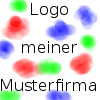
\includegraphics[scale=1]{images/firma-deckblatt.png}}} &
		{\raisebox{\ht\strutbox-\totalheight}{
\includegraphics[height=2.5cm]{images/dhbw.png}}}
	\end{longtable}
	\enlargethispage{20mm}
	\begin{center}
		%\vspace*{12mm}	{\LARGE\textbf \titel }\\
		\vspace*{12mm}  {\LARGE\textbf Logfileanalyse mit Apache\textsuperscript{TM} Hadoop\textsuperscript{\textregistered} MapReduce}\\
		\vspace*{12mm}	{\large\textbf \arbeit}\\
		\vspace*{12mm}	\langdeckblattabschlusshinleitung\\
		\vspace*{3mm}		{\textbf \abschluss}\\
		\vspace*{12mm}	\langartikelstudiengang{} \langstudiengang{} \studiengang\\
    \vspace*{3mm}		\langanderdh{} \dhbw\\
		\vspace*{12mm}	\langvon\\
		\vspace*{3mm}		{\large\textbf \autor}\\
		\vspace*{12mm}	\datumAbgabe\\
	\end{center}
	\vfill
	\begin{spacing}{1.2}
	\begin{tabbing}
		mmmmmmmmmmmmmmmmmmmmmmmmmm             \= \kill
		\textbf{\langdbbearbeitungszeit}       \>  \zeitraum\\
		\textbf{\langdbmatriknr, \langdbkurs}  \>  \martrikelnr, \kurs\\
		\textbf{\langdbfirma}                  \>  \firma, \firmenort\\
		\textbf{\langdbbetreuer}               \>  \betreuer\\
		\textbf{\langdbgutachter}              \>  \gutachter
	\end{tabbing}
	\end{spacing}
\end{titlepage}

	\end{spacing}
	\newpage

	% Sperrvermerk
	%!TEX root = ../dokumentation.tex

\thispagestyle{empty}
% Sperrvermerk direkt hinter Titelseite
\section*{\langsperrvermerk}

\vspace*{2em}

\iflang{de}{%
  Die vorliegende {\arbeit} mit dem Titel {\itshape{} Logfileanalyse mit Apache\textsuperscript{\texttrademark} Hadoop\textsuperscript{\textregistered} MapReduce{}\/} enthält unternehmensinterne bzw. vertrauliche Informationen der {\firma}, ist deshalb mit einem Sperrvermerk versehen und wird ausschließlich zu Prüfungszwecken am Studiengang {\studiengang} der Dualen Hochschule Baden-Württemberg {\dhbw} vorgelegt. Sie ist ausschließlich zur Einsicht durch den zugeteilten Gutachter, die Leitung des Studiengangs und ggf. den Prüfungsausschuss des Studiengangs bestimmt.  Es ist untersagt,
  \begin{itemize}
  \item den Inhalt dieser Arbeit (einschließlich Daten, Abbildungen, Tabellen, Zeichnungen usw.) als Ganzes oder auszugsweise weiterzugeben,
  \item Kopien oder Abschriften dieser Arbeit (einschließlich Daten, Abbildungen, Tabellen, Zeichnungen usw.) als Ganzes oder in Auszügen anzufertigen,
  \item diese Arbeit zu veröffentlichen bzw. digital, elektronisch oder virtuell zur Verfügung zu stellen. 
  \end{itemize}
Jede anderweitige Einsichtnahme und Veröffentlichung – auch von Teilen der Arbeit – bedarf der vorherigen Zustimmung durch den Verfasser und {\firma}.
}

%http://www.ib.dhbw-mannheim.de/fileadmin/ms/bwl-ib/Downloads_alt/Leitfaden_31.05.pdf

\iflang{en}{%
  The {\arbeit} on hand 
  \begin{center}{\itshape{} Logfileanalyse mit Apache{\textsuperscript{TM}} Hadoop\textsuperscript{{\textregistered}} MapReduce{}\/}\end{center} 
   contains internal resp.\ confidential data of {\firma}. It is intended solely for inspection by the assigned examiner, the head of the {\studiengang} department and, if necessary, the Audit Committee \langanderdh{} {\dhbw}. It is strictly forbidden
    \begin{itemize}
    \item to distribute the content of this paper (including data, figures, tables, charts etc.) as a whole or in extracts,
    \item to make copies or transcripts of this paper or of parts of it,
    \item to display this paper or make it available in digital, electronic or virtual form.
    \end{itemize}
  Exceptional cases may be considered through permission granted in written form by the author and {\firma}.
}

\vspace{3em}

\abgabeort, \datumAbgabe
\vspace{4em}

\rule{6cm}{0.4pt}\\
\autor

	\newpage

	% Erklärung
	%!TEX root = ../dokumentation.tex

\thispagestyle{empty}

\section*{\langerklaerung}
% http://www.se.dhbw-mannheim.de/fileadmin/ms/wi/dl_swm/dhbw-ma-wi-organisation-bewertung-bachelorarbeit-v2-00.pdf
\vspace*{2em}

\iflang{de}{%
Ich erkläre hiermit ehrenwörtlich: \\
\begin{enumerate}
\item dass ich meine {\arbeit} mit dem Thema
{\itshape Logfileanalyse mit Apache\textsuperscript{\texttrademark} Hadoop\textsuperscript{\textregistered} MapReduce} ohne fremde Hilfe angefertigt habe;
\item dass ich die Übernahme wörtlicher Zitate aus der Literatur sowie die Verwendung der Gedanken
anderer Autoren an den entsprechenden Stellen innerhalb der Arbeit gekennzeichnet habe;
\item dass ich meine {\arbeit} bei keiner anderen Prüfung vorgelegt habe;
\item dass die eingereichte elektronische Fassung exakt mit der eingereichten schriftlichen Fassung
übereinstimmt.
\end{enumerate}

Ich bin mir bewusst, dass eine falsche Erklärung rechtliche Folgen haben wird.
}

% http://www.ib.dhbw-mannheim.de/fileadmin/ms/bwl-ib/Downloads_alt/Leitfaden_31.05.pdf (S. 52)

\iflang{en}{%
Hereby I solemnly declare:
\begin{enumerate}
\item that this {\arbeit}, titled {\itshape Logfileanalyse mit Apache{\textsuperscript{TM}} Hadoop\textsuperscript{{\textregistered}} MapReduce } is entirely the product of my own scholarly work, unless otherwise indicated in the text or references, or acknowledged below;
\item I have indicated the thoughts adopted directly or indirectly from other sources at the appropriate places within the document;
\item this {\arbeit} has not been submitted either in whole or part, for a degree at this or any other university or institution;
\item I have not published this {\arbeit} in the past; 
\item the printed version is equivalent to the submitted electronic one.
\end{enumerate}
I am aware that a dishonest declaration will entail legal consequences.
}

\vspace{3em}

\abgabeort, \datumAbgabe
\vspace{4em}

\rule{6cm}{0.4pt}\\
\autor

	\newpage

	% Abstract
	%!TEX root = ../dokumentation.tex

\pagestyle{empty}

\iflang{de}{%
% Dieser deutsche Teil wird nur angezeigt, wenn die Sprache auf Deutsch eingestellt ist.
\renewcommand{\abstractname}{\langabstract} % Text für Überschrift

% \begin{otherlanguage}{english} % auskommentieren, wenn Abstract auf Deutsch sein soll
\begin{abstract}
Logfiles beinhalten eine große Menge an Daten deren Analyse bei der Suche nach Fehlern und der Überwachung einer IT Infrastruktur eine große Hilfe sind. Dabei stellen sich mehrere Herausforderungen. Die Erste ist, dass Logfiles textbasiert sind. Der Nachteil hierbei ist, dass, im Vergleich zu einer Datenbank oder einer XML Datei, textbasierte Dateien keine klar auslesbare oder durchsuchbare Struktur besitzen. Die Zweite ist, dass Systeme so viele Informationen wie möglich loggen und dadurch die nützlichen bzw. wichtigen Informationen erst herausgefiltert werden müssen.

Für die Analyse von textbasierten Daten eignet sich sehr gut der MapReduce Algorithmus. Außerdem lässt sich der Algorithmus sehr einfach skalieren und auf mehrere Programmläufe verteilen (Master-Worker). Das Apache Hadoop Projekt stellt sowohl für MapReduce, als auch für die Verwaltung von mehreren Programmläufen, ein Basisframework bereit, mit welchem die Entwicklung eines Analyseprogramms durchgeführt werden soll.

Ziel der Arbeit ist die Entwicklung einer Prototypischen Anwendung zur formatunabhängigen Analyse von Logfiles unter Zuhilfenahme von Apache Hadoop MapReduce.  Die Anwendung soll die bisher vorhandenen Monitoring Systeme innerhalb der Infrastruktur ergänzen, wodurch Informationen über den Zustand des Systems schneller erhoben werden können. Des Weiteren sollen aufkommende Fehler besser erkannt werden, um die Reaktionszeit auf diese zu optimieren.
\end{abstract}
% \end{otherlanguage} % auskommentieren, wenn Abstract auf Deutsch sein soll
}



\iflang{en}{%
% Dieser englische Teil wird nur angezeigt, wenn die Sprache auf Englisch eingestellt ist.
\renewcommand{\abstractname}{\langabstract} % Text für Überschrift

\begin{abstract}
An abstract is a brief summary of a research article, thesis, review, conference proceeding or any in-depth analysis of a particular subject or discipline, and is often used to help the reader quickly ascertain the paper's purpose. When used, an abstract always appears at the beginning of a manuscript, acting as the point-of-entry for any given scientific paper or patent application. Abstracting and indexing services for various academic disciplines are aimed at compiling a body of literature for that particular subject.

The terms précis or synopsis are used in some publications to refer to the same thing that other publications might call an ``abstract''. In ``management'' reports, an executive summary usually contains more information (and often more sensitive information) than the abstract does.

Quelle: \url{http://en.wikipedia.org/wiki/Abstract_(summary)}

\end{abstract}
}
	\newpage

	\pagestyle{plain}		% nur Seitenzahlen im Fuß
	
	%\RedeclareSectionCommand[beforeskip=\kapitelabstand]{chapter} % stellt Abstand vor Kapitelüberschriften ein

	% Inhaltsverzeichnis
	\begin{spacing}{1.1}
		\begingroup
		
			% auskommentieren für Seitenzahlen unter Inhaltsverzeichnis
			\renewcommand*{\chapterpagestyle}{empty}
			\pagestyle{empty}
			
			%\setcounter{tocdepth}{1}
			%für die Anzeige von Unterkapiteln im Inhaltsverzeichnis
			\setcounter{tocdepth}{2}
			
			\tableofcontents
			\clearpage
		\endgroup
	\end{spacing}
	\newpage
	
	\pagenumbering{Roman}

	% Abkürzungsverzeichnis
	\cleardoublepage
	%!TEX root = ../dokumentation.tex

\addchap{\langabkverz}
%nur verwendete Akronyme werden letztlich im Abkürzungsverzeichnis des Dokuments angezeigt
%Verwendung: 
%		\ac{Abk.}   --> fügt die Abkürzung ein, beim ersten Aufruf wird zusätzlich automatisch die ausgeschriebene Version davor eingefügt bzw. in einer Fußnote (hierfür muss in header.tex \usepackage[printonlyused,footnote]{acronym} stehen) dargestellt
%		\acs{Abk.}   -->  fügt die Abkürzung ein
%		\acf{Abk.}   --> fügt die Abkürzung UND die Erklärung ein
%		\acl{Abk.}   --> fügt nur die Erklärung ein
%		\acp{Abk.}  --> gibt Plural aus (angefügtes 's'); das zusätzliche 'p' funktioniert auch bei obigen Befehlen
%	siehe auch: http://golatex.de/wiki/%5Cacronym
%	
\begin{acronym}[YTMMM]
\setlength{\itemsep}{-\parsep}

\acro{API}{Application Programming Interface}
\acro{BDSG}{Bundesdatenschutzgesetz}
\acro{CEP}{Complex Event Processing}
\acro{DEA}{Deterministischer endlicher Automat}
\acrodefplural{DEA}[DEAs]{Deterministische endliche Automaten}
\acro{EDA}{Event Driven Architecture}
\acro{GB}{Gigabyte}
\acro{GFS}{Google File System}
\acro{HDFS}{Hadoop Distributed File System}
\acro{HTTP}{Hypertext Transfer Protocol}
\acro{IDE}{Integrated Development Environment}
\acro{IP}{Internetprotokoll}
\acro{KB}{Kilobyte}
\acro{LTS}{Long Term Support}
\acro{MB}{Megabyte}
\acro{MPI}{Message Passing Interface}
\acro{MRC}{Map Reduce Class}
\acro{NAS}{Network Attached Storage}
\acro{NEA}{Nichtdeterministischer endlicher Automat}
\acrodefplural{NEA}[NEAs]{Nichtdeterministische endliche Automaten}
\acro{NFS}{Network File System}
\acro{OS}{Operating System}
\acro{OSDI}{Operating Systems Design and Implementations}
\acro{PAP}{Programmablaufplan}
\acro{PDF}{Portable Document Format}
\acro{POM}{Project Object Model}
\acro{RFC}{Request for Comments}
\acro{RSA}{Rivest, Shamir und Adleman}
\acro{SAN}{Storage Attached Network}
\acro{SPOF}{Single Point of Failure}
\acro{SSH}{Secure Shell}
\acro{TMG}{Telemediengesetz}
\acro{VM}{Virtuelle Maschine}

\end{acronym}


	% Abbildungsverzeichnis
	\cleardoublepage
	\listoffigures

	%Tabellenverzeichnis
	\cleardoublepage
	\listoftables

	% Quellcodeverzeichnis
	\cleardoublepage
	\lstlistoflistings
	\cleardoublepage

	\pagenumbering{arabic}
	
	\pagestyle{headings}		% Kolumnentitel im Kopf, Seitenzahlen im Fuß

	% Einleitung
	%!TEX root = ../dokumentation.tex

\chapter{Einleitung}\label{cha:Einleitung}
Laut einer Studie des Bitkom e.V. aus dem Jahr 2014 wächst die Datenmenge von Unternehmen seit Jahren exponentiell. Dies ist u.a. auf die verstärkte mobile Internetnutzung zurückzuführen. Für die Analyse dieser Datenmengen werden sog. Big Data Anwendungen benötigt. Die Verarbeitung großer Mengen an Daten unterscheidet sich von der herkömmlichen Datenverarbeitung durch drei Faktoren:

\begin{itemize}
	\item \textbf{Menge:} Keine Begrenzung der Datenmenge für die Verarbeitung
	\item \textbf{Vielfalt:} Daten aus verschiedenen Quellen in unterschiedlichen Formaten
	\item \textbf{Geschwindigkeit:} Die Datenverarbeitung erfolgt oft nahezu in Echtzeit
\end{itemize}

Häufig ist das Ziel die Erkennung neuer Zusammenhänge und Muster. Die gewonnenen Erkenntnisse werden anschließend für Vorhersagen oder Entscheidungsvorlagen verwendet. Die Einsatzgebiete von Big Data Anwendungen umfassen alle Bereiche, in denen größere Datenmengen vorhanden sind.\footcite[Vgl.][S. 3]{Bitkom.2014}

Von diesem Zuwachs an Informationen sind auch Logfiles von Webservern betroffen. Begünstigt durch die wachsenden Geschwindigkeiten des mobilen Internets, werden Webseiten sehr viel häufiger, von einer noch größeren Vielfalt von Geräten aufgerufen. Dabei enthalten Logfiles viele aussagekräftige Informationen, welche sowohl in Echtzeit als auch über längere Zeiträume ausgewertet werden müssen.

Nach einer im Zuge der Studie durchgeführten Umfrage, analysieren 31\% der befragten Unternehmen Logdaten IT-gestützt für Entscheidungsprozesse.\footcite[Vgl.][S. 8]{Bitkom.2014} Ein denkbares Szenario könnte der gezielte Einsatz von Ressourcen zur Verbesserung kritischer Teilsysteme sein. Deren Identifikation könnte durch die Analyse von Logfiles erfolgen.

Eine mögliche Vorgehensweise bei der Analyse von Logfiles, und Kernpunkt dieser Arbeit, stellt das MapReduce Modell in Verbindung mit Apache Hadoop dar.

\newpage
Die in dieser Arbeit dokumentierte Vorgehensweise basiert auf der gegebenen Infrastruktur. Diese wird, um einen Sperrvermerk zu vermeiden, jedoch nicht im Detail beschrieben. Die Funktionsweise der einzelnen Komponenten wurde hinreichend übernommen. Die beschriebenen Grundlagen lassen sich auf vergleichbare Anwendungsfälle übertragen.

%<Kurze Einleitung. Vorstellung der Firma und Abteilung. Allgemeine Heranführung zum Thema und der Brance (IT Umfeld ist groß. Hier sollte klar werden, dass im weiteren Verlauf der Arbeit das Web Umfeld speziell mit Java als Grundlage dient).>

%\section{Motivation}\label{sec:Motivation}


%<Beschreibung warum dieses Thema gewählt wurde für die Arbeit. Eventuell beschreiben was ich mir selbst erhoffe von der Arbeit und welchen Nährwert ich mir wünsche.>

\section{Problemstellung}\label{sec:Problemstellung}
Komplexere Infrastrukturen bestehen aus einer Vielzahl einzelner Systeme (Webserver, Appserver, uvm.). Jede dieser Komponenten generiert Logfiles in unterschiedlichen Formaten. Die Überwachung der Infrastruktur wird durch Monitoring Systeme übernommen. Diese können jedoch nur sehr einfache Analysen durchführen. Die Verarbeitung komplexerer Anfragen ist aktuell nicht möglich. Die Folge ist, dass Informationen oft nur manuell zugänglich sind.

Wird bei einer Komponente ein Fehler festgestellt, so ist die hierfür generierte Benachrichtigung nicht immer aussagekräftig. Die eigentliche Ursache wird erst durch eine händisch durchgeführte Analyse der Logfiles erkennbar.

Um den aktuellen Aufwand bei der Fehlersuche zu verringern, wird eine verbesserte Auswertung der Dateien benötigt, wodurch aussagekräftigere Benachrichtigungen im Problemfall erzeugt werden können, bzw. die Suche nach möglichen Ursachen maschinell durchgeführt werden kann.

%<Genaue Beschreibung der Problemstellung. Was fehlt? Warum fehlt es? Welche Auswirkungen hat das Problem auf die tägliche Arbeit?>

\section{Zielsetzung}\label{sec:Zielsetzung}
Ziel dieser Arbeit ist die Anwendung des MapReduce Modells bei der Entwicklung einer prototypischen Applikation für die Analyse von Logfiles. Bei der Implementierung wird auf das Hadoop Framework der Apache Software Foundation zurückgegriffen.

Die Arbeit soll alle Phasen der Entwicklung dokumentieren und die Funktionsweise von MapReduce vermitteln. Dies bezieht sich nicht nur auf die Implementierung, sondern beinhaltet ebenfalls die theoretischen Hintergründe, sowohl des Modells als auch des gesamten Hadoop Frameworks.

Die fertige Anwendung muss generisch sein und in der Lage sein, unabhängig vom Format eines Logfiles, unterschiedliche Analysen durchführen zu können. Die Parameter der Analyse sollen über Konfigurationsdateien gesteuert werden.

\newpage
Zum Zeitpunkt dieser Arbeit gibt es keinerlei Informationen über die Performance von MapReduce für diesen Anwendungsfall. Sollten die Laufzeiten der Fertigen Anwendung zu hoch sein, müssen die Ergebnisse der Analyse gespeichert und über eine externe Schnittstelle zugänglich gemacht werden.

Die Performance der Anwendung ist durch Anwendungstests festzustellen. Dabei soll die Anzahl verschiedener Fehlercodes in einem Logfile ermittelt werden. Die Menge der Einträge innerhalb der Datei erhöht sich immer nach 10 Programmläufen. Insgesamt sind 100 Analysen durchzuführen. Die ermittelten Laufzeiten sollen Aufschluss über die Performance geben.

\section{Abgrenzung}\label{sec:Abgrenzung}
Nicht Teil der Arbeit ist die Installation und Konfiguration des Ressourcenmanagement und der automatischen Skallierung von Hadoop. Es wird nur eine einfache Single Node Installation vorgenommen und beschrieben. Ebenfalls nicht teil der Arbeit ist die Impelmentierung eines Checkskriptes für ein Monitoringtool.

Ebenfalls nicht teil der Arbeit ist die Absicherung der Hadoop Infrastruktur oder andere Sicherheitsfragen bei der Entwicklung von MapReduce Anwendungen. Ein Hinweis auf mögliche Schwachstellen reicht hier aus.

Logfiles können Personenbezogene Daten enthalten, welche nach §3 Abs. 1 \ac{BDSG} geschützt werden müssen\footcite[§3 Abs. 1 BDSG,][]{BDSG3.1990} (Potenziell Personenbezogen, da nicht ersichtlich ist, ob eine \ac{IP}-Adresse statisch oder dynamisch ist). Die Speicherung von z.B. der \ac{IP}-Adresse ist daher nur gestattet, wenn der Anwender zustimmt, oder ein Grund für die Speicherung vorliegt, welcher §15 \ac{TMG} genügt.\footcite[§15 TMG,][]{TMG15.2007}  Da es sich bei dem im Zuge dieser Arbeit entwickelten Programm um eine prototypische Anwendung handelt, sind die Datenschutzrichtlinien nicht Teil der Arbeit und werden daher nicht betrachtet.

%Was soll NICHT Teil der Arbeit sein? Dabei unbedingt beschreiben das die serverseitige Konfiguration von Hadoop und YARN und das Aufsetzung von Clustern ignoriert wird. Dadurch soll klar werden, dass der Fokus auf der Anwendung des Algorithmus auf einen konkreten Fall liegt.
	
	% Theoretische Grundlagen
	%!TEX root = ../dokumentation.tex

\chapter{Theoretische Grundlagen}\label{cha:Grundlagen}
Für das bessere Verständnis des Themas soll dieses Kapitel die relevanten, theoretischen Grundlagen vermitteln,  und an das Kernthema heranführen. Dabei wird zunächst geklärt, worum es sich bei der Überwachung von IT-Infrastrukturen handelt, und soll Antworten auf Fragen wie "`Warum werden diese überwacht?"', "`Welche Komponenten sind zu unterscheiden?"' und "`Welche Technologien werden eingesetzt?"' geben. Danach soll der Begriff Logfiles genauer definiert werden, bevor die Funktionalität von MapReduce und Hadoop erläutert wird.

%TODO: Einleitung überarbeiten
<Einleitung in das Kapitel noch nicht wirklich rund. Überarbeiten!>

%Kurze Einleitung in das Kapitel. Beschreiben warum die Grundlagen notwendig sind. Auch darüber schreiben, dass nicht ALLE Grundlagen sondern lediglich die für das Verständnis der Arbeit notwendigen erklärt werden.

\section{Überwachung von IT-Infrastrukturen}\label{sec:UeberwachungIT}
Ziel der Überwachung ist es, durch Extraktion von Informationen und überprüfen von Komponenten, Aussagen über den Zustand einer oder mehrerer Komponenten innerhalb einer IT-Infrastruktur zu erhalten. Die durch die Überwachung erhobenen Basis-Informationen werden zur Optimierung der Performance und Verfügbarkeit eines Dienstes eingesetzt.

Nach Salm gibt es drei Arten von Komponenten die es zu unterscheiden gilt:

\begin{itemize}
	\item Netzwerk, um eine ausreichende Bandbreite und bestehende Übertragung zu sichern
	\item Ressourcen, um eine effiziente Lastverteilung innerhalb der Infrastruktur zu gewährleisten
	\item Anwendung, um Anwender schnellen, unkomplizierten Zugriff zu ermöglichen
\end{itemize}

Überwachungssysteme zeigen Administratoren die Up- und Downtime, sowie die Auslastung, von Soft- und Hardware an.\footcite[Vgl.][S. 8]{Salm.2007}

Um Aussagen über den Zustand einer Komponente treffen zu können, analysiert das Überwachungssystem eine Vielzahl von Informationen. Dabei werden unterschiedliche Techniken eingesetzt von einfachen Standard-Unix-Kommandozeilen-Tools bis hin zu intelligenten Agenten.

Diese Agenten werden auf der Zielkomponente installiert und sind als Hintergrundanwendung dauerhaft aktiv um immer die aktuellsten Informationen an das Überwachungssystem zu übermitteln.

Um eine hohe Qualität der Daten zu gewährleisten, werden die Agenten, entweder direkt oder über eine externe Schnittstelle, so konfiguriert, dass sie nur die Informationen ermitteln und übertragen, welche für das Überwachungssystem relevant sind. Agenten können auch eine direktere Rolle bei der Überwachung von Komponenten übernehmen, indem sie, anstatt oder zusätzlich zu den Informationen, die Daten selbst interpretieren, um Meldungen an das Überwachungssystem zu übermitteln.

In beiden fällen kombinieren Agenten selbst ermittelte Informationen mit bereits vorhandenen. Zu den selbst ermittelten Daten gehören unter anderem CPU und RAM Auslastung oder offene Ports. Bereits vorhandene Informationen können durch auf der Komponente laufende Software, oder durch die Komponente selbst, erzeugt werden.

Speziell Webseiten und deren Infrastrukturen, ist die Überwachung ein signifikanter Punkt bei der Qualitätssicherung. Die Verfügbarkeit eines Systems ist oft Teil von Dienstleistungsverträgen. Aus diesem Grund setzen IT-Dienstleister auf Monitoring Systeme wie \gls{Nagios} oder \gls{Zabbix}, um Informationen über die von ihnen administrierten Systeme zu erhalten. Auf allen zu überwachenden Systemen werden die entsprechenden Agenten installiert und aktiviert. Danach kann das Hauptsystem über die Agenten alle benötigten Informationen beziehen.

Von besonderem Interesse sind hier Logfiles. Aus ihnen lassen sich viele Informationen über den Zustand eines Systems ausgelesen. Dabei handelt es sich sowohl um Real- oder Near-Time, als auch historische Informationen.

%TODO: Überleitung zu Logfiles schreiben aus fokusieren auf web und monitoring systemen
%<Kurze Fokusierung auf Online Service. Welche Informationen werden hier im speziellen benötigt. Erwähnen von Monitoring Systemen. Funktion von Agenten, im zusammenspiel mit Monitoring Systemen, bei der analyse von Logfiles beschreiben und daraus die Überleitung zu Logfiles ableiten>

%Worum geht es bei der Überwachung? Was ist das Ziel? Warum braucht man eine Überwachung? Wie sieht diese i.d.R. Aus? Welche Kernpunkte gibt es in der Überwachung? \\
%Hier sollte die Überleitung zum nächsten Kapitel kommen d.h. Logfiles werden als letztes behandelt in diesem Kapitel, damit der Übergang sauber ist.

\section{Bedeutung von Logfiles}\label{sec:BedeutungVonLogfiles}
Nach Baur und Blasius bezeichnen Logfiles (oder auch Protokolldateien) \flqq [...] automatisch erstellte Dateien [..], in denen bestimmte Ereignisse elektronisch aufgezeichnet werden.\frqq\footcite[S. 847]{Baur.2014} Dabei werden sowohl negative wie auch positive Ereignisse protokolliert.

Bei Web-Servern, welche mit Apache \acs{HTTP} Server (später Apache) unter Linux betrieben werden, stellen syslog von Linux, sowie Error- und Access-Log von Apache, die Grundlage zur Überwachung des Servers. Sie lassen sich sehr einfach durch die in \autoref{sec:UeberwachungIT} beschriebenen Agenten überwachen, da sie einem klar vorgegebenen Standard folgen.

Im syslog von Linux werden alle Ereignisse protokolliert, welche im direkten Zusammenhang mit dem System stehen. Die Einträge folgen dabei der im \ac{RFC} 5424\footcite[RFC 5424,][]{RFC5424.2009} festgehaltenen Beschreibung (Da es sich bei RFC um keine offizielle Norm handelt, handelt es sich lediglich um eine Beschreibung, nicht um einen Standard).

Das Apache-Error-Log enthält diagnostische Informationen und protokolliert alle Fehler, welche bei der Verarbeitung einer Anfrage auftreten. \autoref{lst:BeispieleintragApacheErrorLog} zeigt, wie ein Eintrag in einem Error-Log aussehen könnte. Es lässt sich klar erkennen, wann der Fehler aufgetreten ist, was fehlgeschlagen ist und welches Modul betroffen ist. Ebenfalls sichtbar ist die \ac{IP}-Adresse des Clients, bei dem der Fehler aufgetreten ist. Die Einträge des Error-Logs entsprechen keiner Norm oder \ac{RFC} Beschreibung. Sie können nach der Installation individuell angepasst werden.\footcite[Vgl.][]{ApacheErrorLog.2015} \\

\begin{lstlisting}[caption=Beispieleintrag für ein Apache-Error-Log,label=lst:BeispieleintragApacheErrorLog]
[Fri Jun 12 10:42:29.902022 2015] ERROR [pid 35708:tid 4328636416] [client 192.168.172.15] File does not exist: /usr/local/apache2/htdocs/favicon.ico
\end{lstlisting}

Im Apache-Access-Log werden alle Anfragen an den Server protokolliert. Dabei wird gespeichert von welcher \ac{IP}-Adresse die Anfrage kam, wann die Anfrage gestartet wurde, welcher Art die Anfrage war und welcher Pfad angefragt wurde, sowie welcher Statuscode zurückgegeben wurde und wie groß die Antwort des Servers war (siehe \autoref{lst:BeispieleintragApacheAccessLog}). \\

\begin{lstlisting}[caption=Beispieleintrag für ein Apache-Access-Log,label=lst:BeispieleintragApacheAccessLog]
192.168.172.15 - Max [11/Jun/2015:13:55:36 -0700] "GET /dummy.gif HTTP/1.0" 200 2326
\end{lstlisting}

Wie beim Error-Log können die Einträge angepasst werden und folgen somit keiner Norm oder \ac{RFC}. Die Beispiele zeigen ebenfalls, wie unterschiedlich die Einträge für zwei Logfiles des gleichen Systems sein können.\footcite[Vgl.][]{ApacheAccessLog.2015}

Da es sich bei \ac{IP}-Adressen potenziell um Personenbezogenen Daten handelt, ist diese nach §3 Abs. 1 \ac{BDSG} geschützt\footcite[§3 Abs. 1 BDSG,][]{BDSG3.1990} (Potenziell Personenbezogen, da nicht ersichtlich ist, ob eine \ac{IP}-Adresse statisch oder dynamisch ist). Die Speicherung der \ac{IP}-Adresse ist daher nur gestattet, wenn der Anwender zustimmt, oder ein Grund für die Speicherung vorliegt, welcher §15 \ac{TMG} genügt.\footcite[§15 TMG,][]{TMG15.2007} Ist dies nicht der Fall, darf die \ac{IP} nicht Teil des Protokolleintrags sein. Die Standardeinstellung muss entsprechend verändert werden.

Da es sich bei dem im Zuge dieser Arbeit entwickelten Programm um eine prototypische Anwendung handelt, können die Datenschutzrichtlinien vorerst vernachlässigt werden. Es geht primär um die Anwendung eines Modells auf einen konkreten Fall.

Wie gezeigt wurde, gibt es keinen einheitlichen Standard für die Notation innerhalb von Logfiles. Dieser Umstand hat zur Folge, dass nur die üblichen Logfiles wie Error- oder Access-Log, über Agenten ausgewertet werden können, solange deren Notation nicht verändert wurde. Um dennoch Informationen über den Zustand eines Systems oder einzelner Module automatisiert zu erhalten, müssen entsprechende Anwendungen geschrieben werden. Da es sich hierbei um eine sehr große Menge an textbasierten Daten handelt, eignet sich hierfür besonders das MapReduce-Modell.

%<Zusammenfassung am ende des Kapitels. Aufzeigen das Logfiles unterschiedliche Notation besitzen und keinem einheitlichen Standard folgen. Erwähnen das die üblichen Logs trotz allem durch Agenten auswertbar sind, die Logs um die es später geht jedoch nicht. Aus dieser Aussage die verwendung von MapReduce begründen und daraus die Überleitung zu MapReduce bilden>

%Was sind Logfiles im allgemeinen? Was ist die Funktion eines Logfiles? Gibt es Standards? Wenn ja welche und wie sehen die aus? Werden die Standards im weiteren Verlauf der Arbeit noch einmal relevant sein (Ja/Nein begründen und erläutern)?

\section{Einführung in MapReduce}\label{sec:EinführungInMapReduce}
Die Google Mitarbeiter Jeffrey Dean und Sanjar Ghemawat veröffentlichten 2004 eine Arbeit, in welcher sie einen neuen Ansatz zur Verarbeitung von großen, unstrukturierten Daten beschrieben. Das in der Arbeit beschriebene Modell wurde als \textit{Map-Reduce} bezeichnet. Dabei wurde nicht nur beschrieben, wie man große Datenmengen durchsucht, auswertet und in Schlüssel-Wert-Paaren zusammenfasst. Die Clusterung von Jobs auf \gls{Commodity-Hardware} waren ebenfalls ein Bestandteil der Arbeit. Freiknecht schreibt weiter, dass diese Arbeit als Ursprung des Algorithmus bezeichnet wird, und somit Implementierungen wie Hadoop, Disco oder BashReduce inspiriert hat.\footcite[Vgl.][S. 42]{Freiknecht.2014}

Ein MapReduce Programm lässt sich i.d.R. in drei Bereiche unterteilen. Der Map-Phase, in welcher die Schlüssel-Wert-Paare aus den Eingabedaten erzeugt werden, der Combine-Phase, zur Aggregation der Paare, sowie der Reduce-Phase, in welcher die Daten ausgedünnt werden, bis nur noch ein Wert pro Schlüssel vorhanden ist (siehe \autoref{fig:DreiPhasenMapReduce}).

\begin{figure}[h]
	\centering
	
\includegraphics[width=.8\textwidth]{MapReduce_001.png}
	\caption{Die drei Phasen eines Map-Reduce-Prozesses\footnotemark}
	\label{fig:DreiPhasenMapReduce}
\end{figure}
\footnotetext{\cite[S. 42.]{Freiknecht.2014}}

Die Stärke von MapReduce, liegt in der Kombination von sequentieller und paralleler Verarbeitung. Die einzelnen Phasen von MapReduce werden sequentiell ausgeführt. Die Combine- oder Reduce-Phase kann nicht beginnen, bevor die Map-Phase abgeschlossen ist. Innerhalb der Phasen können die Aufgaben jedoch auf mehrere Instanzen verteilt und parallel verarbeitet werden. Diese Form der Verarbeitung entspricht dem Master-Worker-Modell.\footcite[Vgl.][S.1 f]{Karloff.2010}

Speziell bei der Parallelisierung von Tasks, welche wenig bis keine Abhängigkeit voneinander aufweise, stellt dieses Modell ein ideales Hilfsmittel dar. Die zentralen Elemente des Schemas bildet ein Master und $n$ Worker. Der Master startet die Verarbeitung, indem er ein gegebenes Problem aufarbeitet und eine Sammlung von Tasks erzeugt.  Die Tasks werden vom Master an die ihm bekannten Worker verteilt (Worker werden entweder vom Master selbst erzeugt oder melden sich bei diesem an). Die Worker arbeiten parallel und senden einen Statuscode an den Master, sobald der Task vollständig bearbeitet wurde (oder der Worker in einen Fehler läuft).\footcite[Vgl.][S. 80 ff]{Fey.2008} \autoref{fig:MasterWorkerInMR} zeigt die Anwendung des Master-Worker-Modells auf ein MapReduce Programm.

\begin{figure}[h]
	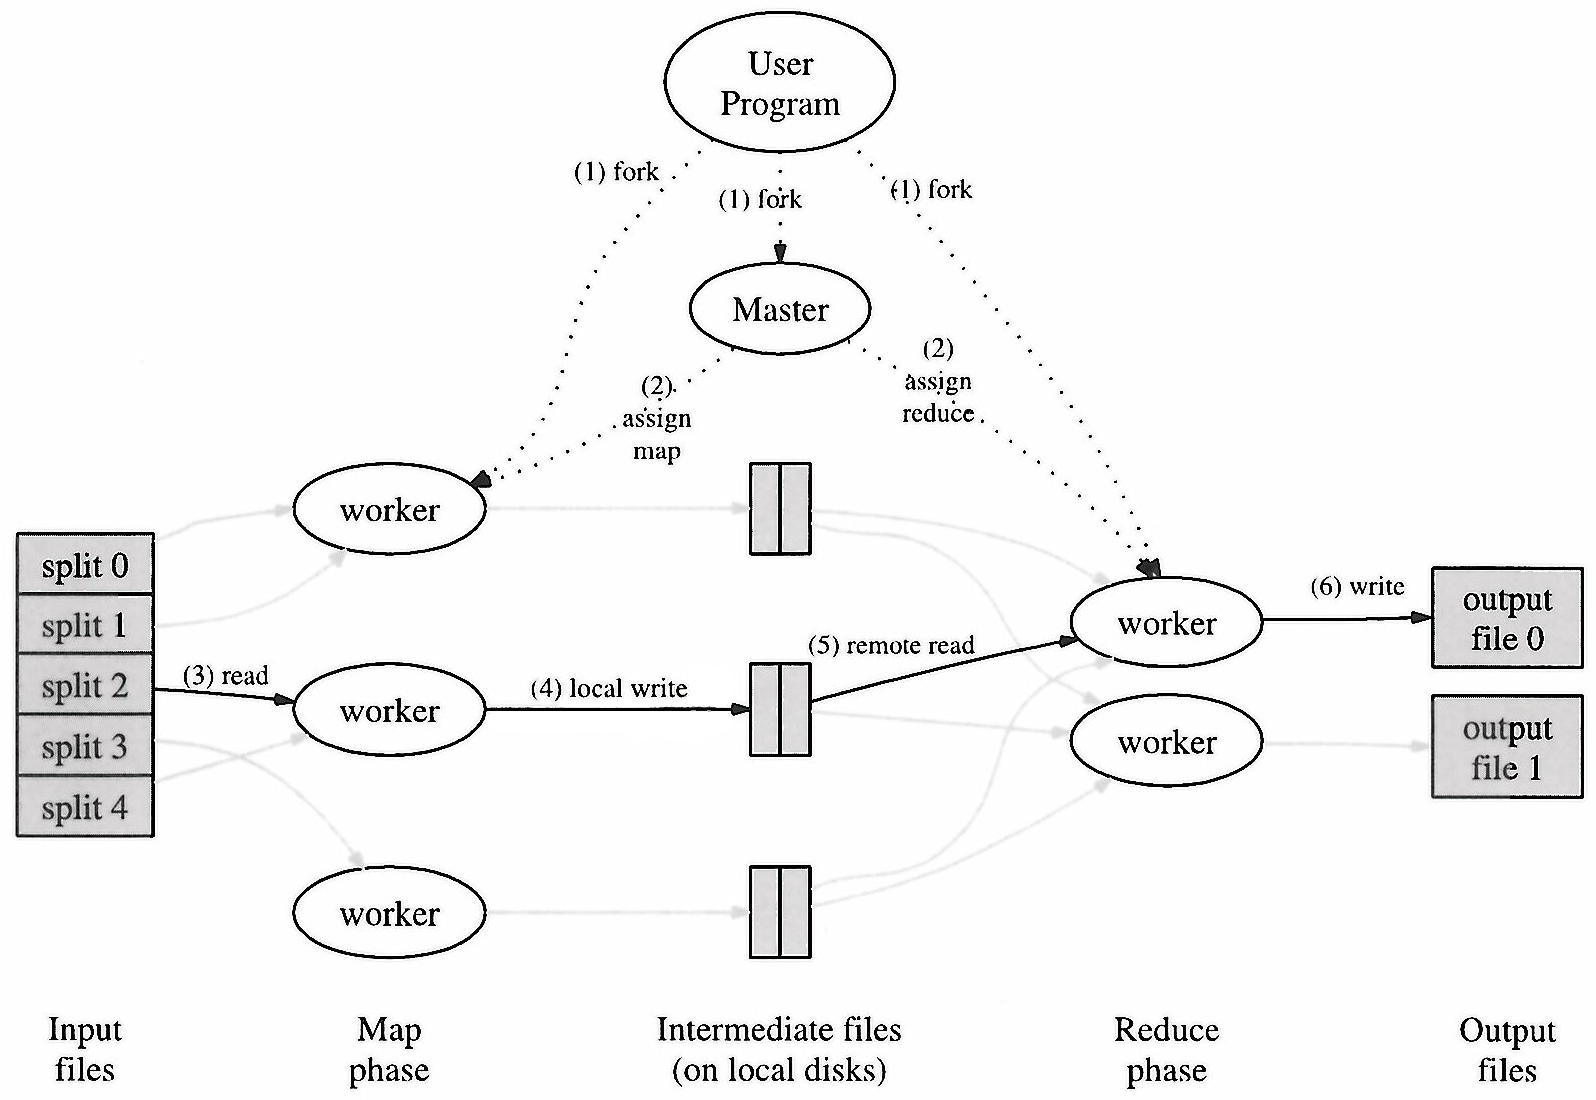
\includegraphics[width=1\textwidth]{MasterWorkerMR.png}
	\caption{Master-Worker in MapReduce\footnotemark}
	\label{fig:MasterWorkerInMR}
\end{figure}
\footnotetext{\cite[S. 3.]{Dean.2004}}

Im folgenden wird MapReduce zunächst formal definiert. Die Grundlage der Definition bildet das durch Karloff, Suri und Vassilvitskii beschriebene \ac{MRC} Model.\footcite[S. 3 f]{Karloff.2010} Danach soll die Funktionsweise anhand eines Beispiels weiter verdeutlicht werden.

\subsection{Formale Beschreibung von MapReduce}\label{subsec:FormaleBeschreibung}
Da es sich bei MapReduce um ein Modell zur Verarbeitung von Daten handelt, und nicht um einen Algorithmus, wird die durch Karloff et al. beschriebene \ac{MRC} verwendet, um eine Grundlage für die formale Definition zu haben. Dabei werden die drei Karakteristiken Funktion, Ausführungszeit und Speicherauslastung beschrieben.

Im Zentrum der Datenverarbeitung mit MapReduce steht das Schlüssel-Wert-Paar, welches als ein String Tupel $\langle k; v \rangle$, mit dem Schlüssel $k$ und dem dazu gehörenden Wert $v$. Die Eingabe für eine \ac{MRC} Maschine ist eine Liste von Schlüssel-Wert-Paaren $\langle k_i, v_i \rangle_{i=1}^{\mathbb{N}}$ mit einer Gesamtgröße im Speicher von $\sum_{i=1}^{\mathbb{N}}|k_i|+|v_i|$.

Die Map Funktion verarbeitet einen Tupel $\langle k; v \rangle$ zu einer Liste von neuen Schlüssel-Wert-Paaren $\langle k_1; v_1 \rangle, \langle k_2; v_2 \rangle, \dots, \langle k_n; v_n \rangle$.

Die Reduce Funktion erhält als Eingabeparameter einen Schlüssel $k$ sowie eine Sequenz von Werten $v_1, v_2, \dots, v_n$. Aus diesen erzeugt die Funktion eine Liste von Schlüssel-Wert-Paaren $\langle k; v_{k,1} \rangle, \langle k; v_{k,2} \rangle, \dots, \langle k; v_{k,n} \rangle$. Die Schlüssel der Tupel in der erzeugten Liste ist identisch mit dem Schlüssel, welcher an die Reduce Funktion übergeben wurde.

Aus diesen beiden Definitionen folgt, dass die Map Funktion Schlüssel nach belieben manipulieren kann. Für Reduce sind die Schlüssel jedoch unveränderlich.

Die Ausführung von MapReduce lässt sich wie folgt definieren. Sei $M$ die Menge aller Map und Reduce Funktionen $\langle \mu_1, \rho_1, \mu_2, \rho_2, \dots, \mu_R, \rho_R \rangle$ und $U_0$ eine Liste von Tupeln $\langle k; v \rangle$, dann gilt für die Ausführung von $M$ auf die Daten $U_0$:

Für $r = 1, 2, \dots, R$:

\begin{enumerate}
	\item \textbf{MAP:} $\forall \langle k; v \rangle \in U_{r-1}$ führe $\mu_r \in M$ mit $\langle k; v \rangle$ aus. Die Funktion erzeugt eine Liste neuer Tupel $\langle k_1; v_1 \rangle, \langle k_2; v_2 \rangle, \dots, \langle k_n; v_n \rangle$. Sei $U_r^{\prime}$ die Ausgabe für eine Eingabe $\langle k; v \rangle$, dann gilt: $U_r^{\prime} = \bigcup_{\langle k; v \rangle \in U_{r-1}} \mu_r(\langle k; v\rangle)$.
	\item \textbf{COMBINE:} $\forall k$ erzeuge Liste $V_{k,r}$ mit den Werten $v_i$, so dass gilt $\langle k; v_i \rangle \in U_r^{\prime}$.
	\item \textbf{REDUCE:} $\forall k$, übergebe $k$ und eine willkürliche Permutation von $V_{k,r}$ in eine Instanz von Reducer $\rho_r \in M$ zur Ausführung. Dieser erzeugt eine Liste von Tupeln $\langle k; v_1^{\prime} \rangle, \langle k; v_2^{\prime} \rangle, \dots, \langle k; v_n^{\prime} \rangle$. Sei $U_r$ die Ausgabe für die Eingabe $\langle k; V_{k,r} \rangle$, \\ dann gilt: $U_r = \bigcup_k \rho(\langle k; V_{k,r}\rangle)$.
\end{enumerate}

Die Verarbeitung wird beendet, wenn der letzte Reducer $\rho_R$ beendet wird. In der Definition wird die Möglichkeit zur Parallelisierung, der sequentiell ausgeführten Funktionen Map und Reduce deutlich. Sowohl Mapper als auch Reducer verarbeiten immer nur einen Tupel zeitgleich. Es können also mehrere Instanzen von $\mu_r$ und $\rho_r$ gestartet werden.\footcite[Vgl.][S. 2 f]{Karloff.2010}

Die Ausführungszeit von MapReduce kann nicht spezifiziert werden ohne ein Wissen über den Inhalt der Funktionen. Die Effizient hängt von den in den Funktionen angewandten Algorithmen ab. Allgemein lässt sich folgende Ausführungszeit definieren: Teilt man die Map-Phase in $M$ Teile und die Reduce-Phase in $R$ Teile, dann lässt sich allgemein eine Ausführungszeit von $O(M+R)$ festlegen. Für die Speicherauslastung gilt dabei eine maximale Auslastung von $O(M \times R)$.\footcite[Vgl.][S. 5]{Dean.2004}

\subsection{Beispielanwendung von MapReduce}\label{subsec:Beispielanwendung}
Die formale Definition von MapReduce soll nun anhand eines einfachen Beispiels verdeutlicht werden. Dazu wird auf eine Beispielanalyse aus dem Buch "`Hadoop - Zuverlässig, verteilte und skalierbare Big-Data-Anwendungen"' von Ramon Wartala zurückgegriffen.

In seinem Beispiel will Wartala aufzeigen, wie, ohne die volle Funktionalität der Hadoop-Api zu nutzen und unter Verwendung von Standard-Unix-Kommandozeilen-Tools wie \textit{grep}, \textit{sort}, \textit{cat} und \textit{awk}, aus einer CSV-Datei eine spezifische Information extrahiert werden kann.

\autoref{tbl:Beispieldaten} zeigt die in seinem Beispiel verwendeten Daten. Dabei handelt es sich um die Anzahl der im Hafen Hamburg von 2004 bis 2011 umgeschlagenen Container pro Monat. Um die Verarbeitung für das Beispiel zu vereinfachen, wurde aus den Daten eine dreispaltige CSV-Datei erzeugt im Format \textit{Jahr;Monat;Container-Umschlag}.

\pagebreak
\begin{table}[h]
	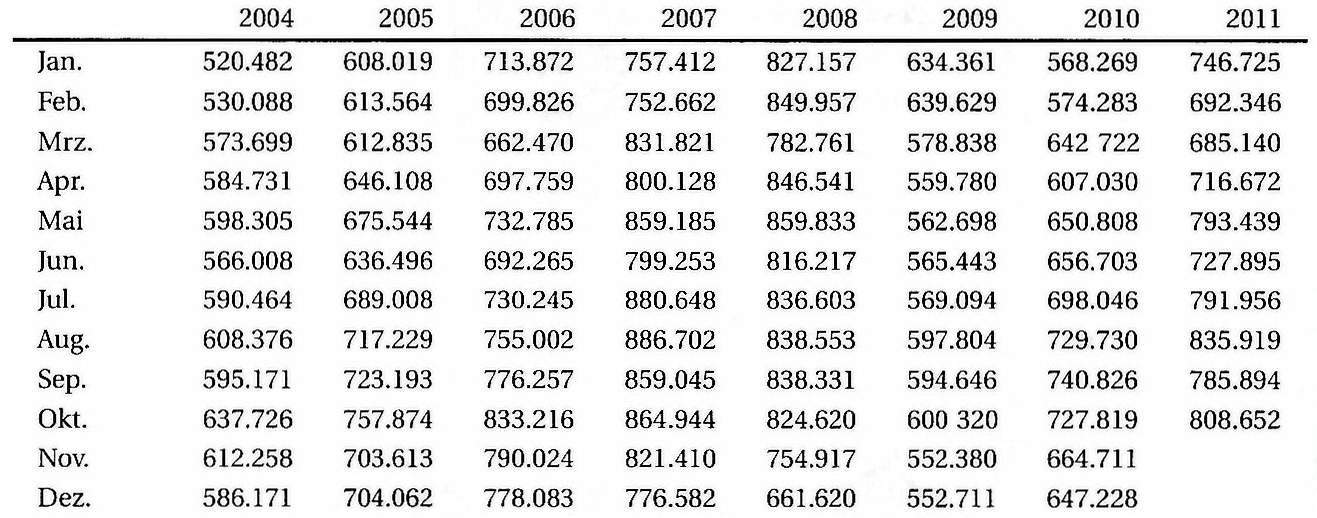
\includegraphics[width=1\textwidth]{Beispieldaten.png}
	\caption{Beispieldaten: Anzahl umgeschlagener Container\footnotemark}
	\label{tbl:Beispieldaten}
\end{table}
\footnotetext{\cite[S. 26.]{Wartala.2012}}

Die Information, welche mit MapReduce ermittelt werden soll, ist der Monat im Jahr 2004 mit den meisten umgeschlagenen Containern. Dieser Task lässt sich, unter Verwendung der erwähnten Unix-Tools, in drei Teilaufgaben separieren. Als erstes werden mit den \textit{grep}-Befehl alle Zeilen ausgegeben, welche aus dem Jahr 2004 stammen (siehe \autoref{lis:Grep2004}). Dieser Schritt repräsentiert den Mapper für dieses Beispiel. \\

\begin{lstlisting}[language=bash, caption=Befehl zur Anzeige aller Zeilen mit Jahr 2004, title=\autoref*{lis:Grep2004}: Befehl zur Anzeige aller Zeilen mit Jahr 2004\protect\footnotemark, label=lis:Grep2004]
grep 2004
\end{lstlisting}
\footnotetext{\cite[S. 27.]{Wartala.2012}}

Danach werden die Zeilen nach der dritten Spalte sortiert (Spalten wurden mit ; getrennt, siehe \autoref{lis:SortiereZeilen}). Dieser Befehl repräsentiert die Combine-Phase des Modells. \\

\begin{lstlisting}[language=bash, caption=Befehl zur Sortierung der Zeilen nach der dritten Spalte, title=\autoref*{lis:SortiereZeilen}: Befehl zur Sortierung der Zeilen nach der dritten Spalte\protect\footnotemark, label=lis:SortiereZeilen]
sort -t ';' -k +3 -r
\end{lstlisting}
\footnotetext{\cite[S. 27.]{Wartala.2012}}

Zuletzt wird die maximale Anzahl der Container bestimmt und das Jahr sowie der Monat und die Anzahl ausgegeben (siehe \autoref{lis:AusgabeBeispiel}). Dieser letzte Schritt in diesem Beispiel steht für den Reducer. \\

\begin{lstlisting}[language=bash, caption=Ausgabe des Beispielprogramms, title=\autoref*{lis:AusgabeBeispiel}: Ausgabe des Beispielprogramms\protect\footnotemark, label=lis:AusgabeBeispiel]
awk 'max== "" || $3 > max {max=$3;jahr=$1;monat=$2} END { print "jahr:" jahr; print "monat:" monat; print "anzahl:" max;}' FS=";"
\end{lstlisting}
\footnotetext{\cite[S. 27.]{Wartala.2012}}

Mit Hilfe der Unix-Befehls-Pipeline lassen sich alle Befehle auf eine Zieldatei Anwenden (siehe \autoref{lis:VollständigerBefehl}). Das Ergebnis wird in die Datei maximum\_umschlag.txt geschrieben.\footcite[Vgl.][S. 26 ff]{Wartala.2012} \\

\begin{lstlisting}[language=bash, caption=Vollständiger Befehl zur Auswertung der Beispieldaten, title=\autoref*{lis:VollständigerBefehl}: Vollständiger Befehl zur Auswertung der Beispieldaten\protect\footnotemark, label=lis:VollständigerBefehl]
cat container_umschlag.csv | grep 2004 | sort -t ';' -k +3 -r | awk 'max== "" || $3 > max {max=$3;jahr=$1;monat=$2} END { print "jahr:" jahr; print "monat:" monat; print "anzahl:" max;}' FS=";" | cat > maximum_umschlag.txt
\end{lstlisting}
\footnotetext{\cite[S. 28.]{Wartala.2012}}

Hier wird deutlich, dass es sich bei MapReduce nicht um einen Algorithmus, sondern um ein Vorgehensmodell handelt. Es geht lediglich darum, die Datenverarbeitung so effizient wie möglich sowohl parallel als auch seriell durchzuführen. Wie das Beispiel zeigt, lässt sich dieses Vorgehen auch sehr minimalistisch anwenden.

Für die Anwendung von MapReduce auf komplexere bzw. größere Daten reicht diese vereinfachte Form nicht mehr aus. Eine Lösung hierfür bietet das Hadoop Framework.

%<Noch ein paar sätze zur anwendung auf komplexere daten. Daraus die Überleitung zum nächsten Kapitel über Hadoop und das Framework schaffen>

%Woher kommt MapReduce? Wie funktioniert MapReduce? Stärken/Schwächen aufzeigen. Versuchen den Algorithmus mathematisch zu beschreiben ($O(n)$ Methode, Mengenleere). Hierfür muss noch Literatur gesucht werden. Bisher nur mathematische Beschreibungen im Internet gefunden.

%TODO: Einleitung ändern. Nicht direkt mit Zitat beginnen. Eher etwas in die richtung "Wartala sagt..." oder so
\section{Was ist Hadoop?}\label{sec:WasIstHadoop}
\flqq Kurz gesagt: Hadoop ist ein freies, Java-basiertes Open-Source-Framework für die skalierbare und verteilte Verarbeitung großer Datenmengen auf vielen Rechnern innerhalb eines Netzwerks.\frqq\footcite[S. 21]{Wartala.2012}

Die Entwicklung begann im Jahr 2004 durch den Programmierer Doug Cutting, nachdem dieser, im Rahmen des 6. Symposiums \ac{OSDI}, den Vortrag "`MapReduce - Simplified Data Processing on Large Clusters"', von den Google Mitarbeitern Jeffrey Dean und Sanjay Ghemawat, gehört hatte.

Zu diesem Zeitpunkt arbeitete Cutting an seinem Suchmaschinenprojekt mit dem Namen "`Nutch"', welches bereits 2002 ins leben gerufen wurde. Sein Ziel war eine leistungsfähige und konkurrenzfähige Softwarearchitektur, die es mit kommerziellen Suchmaschinen aufnehmen konnte. Bis 2004 konnte Nutch bereits 100 Mio. Webseiten mit nur vier Rechnerknoten indexieren.

Um jedoch das gesamte World Wide Web indexieren zu können, suchte Cutting gemeinsam mit der Nutch-Community nach einer Möglichkeit, die zugrundeliegende Architektur noch skalierbarer zu machen. Nach dem Vortrag bei der \ac{OSDI} fand Cutting eine passende Systemarchitektur in einem ebenfalls durch Dean und Ghemawat veröffentlichten Ansatz.\footcite[Näheres siehe][]{Dean.2004}

Gemeinsam mit zwei Teilzeit-Programmierern implementierte er ein, durch das Google Dateisystem \ac{GFS} inspiriertes, verteiltes Dateisystem, um darauf den MapReduce-Ansatz unter Nutch zu realisieren. 2006 wechselte Cutting zu Yahoo!. Das Dateisystem und MapReduce-Framework wurde aus Nutch extrahiert und in das eigenständige Apache-Projekt Hadoop überführt. Heute wird Hadoop in einer Reihe von Unternehmen produktiv eingesetzt, darunter Yahoo!, IBM und Microsoft.\footnote{Referenzzahlen für Unternehmen, die Hadoop einsetzen, unter:\\ \url{http://wiki.apache.org/hadoop/PoweredBy}}

Hadoop besteht aus zwei Kernkomponenten. Dem verteilten Dateisystem \ac{HDFS} und dem MapReduce-Framework. Dabei wird keine spezielle Servertechnik benötigt. Hadoop lässt sich sehr leicht auf Standardhardware betreiben.\footcite[Vgl.][S. 19-22]{Wartala.2012}

Die einzelnen Komponenten sind unabhängig voneinander einsetzbar. Eine große Rolle spielt bei Hadoop das Konzept der Datenlokalität. Entgegen dem normalen vorgehen, bei welchem einem Programm die Daten zu Verfügung gestellt werden, wird bei Hadoop das Programm zur Ausführung im Cluster verteilt. Da es sich bei Hadoop i.d.R. um Anwendungen im Big Data Bereich handelt, macht es Sinn, da die Anwendung wesentlich kleiner und somit schneller zu übertragen ist, als die Daten.\footcite[Vgl.][S. 20]{Freiknecht.2014}

\subsection{Das verteilte Dateisystem HDFS}\label{subsec:DasVerteilteDateisystemHDFS}
Den Kern, und somit die wichtigste Funktion von Hadoop, Bilder das Dateisystem. Aktuell werden Daten zum Großteil in relationalen Datenbanken gespeichert. Parallel existiert noch die Möglichkeit, Daten ohne Relation direkt auf einem herkömmlichen Dateisystem abzulegen (sog. Flat-Files). Da die Verteilung und Verwaltung großer Datenmengen in einem Cluster sehr aufwändig ist, wurde, angelehnt an das \ac{GFS}, \ac{HDFS} entwickelt. Dabei wurden die folgenden Anforderungen an das Design des Dateisystems gestellt:

\begin{itemize}
	\item Betrieb auf \gls{Commodity-Hardware}
	\item Ausfallsicherheit einzelner Knoten
	\item Speicherung und Verarbeitung großer Datenmengen
	\item Einfache Skalierbarkeit\footcite[Vgl.][S. 21]{Freiknecht.2014}
\end{itemize}

Dabei macht sich \ac{HDFS} zusätzlich die bekannten Eigenschaften verteilter Dateisysteme zunutze. Der \textit{Parallelisierung}, dem gleichzeitigen Lesen und Schreiben von Dateien, verteilt im Netz auf vielen Rechnern. Der \textit{Cluster-lokalen Verarbeitung}, bei der die Verarbeitungsprozesse auf den Knoten im Cluster ausgeführt werden, welche die Daten halten, um die Kommunikation im Netzwerk so gering wie möglich zu halten. Zuletzt dem \textit{Failover}-Prinzip, bei dem die Daten auf die einzelnen Knoten blockweise und gleichmäßig verteilt werden.

Mittels \ac{HDFS} ist Hadoop in der lage, große Datenmengen auf kostengünstiger Standarthardware zu speichern, im Vergleich zu kostspieligen Speichernetzwerken (\ac{SAN} oder \ac{NAS}). 

Die Architektur von \ac{HDFS} entspricht einem Master-Slave-System. Die verschiedenen Aufgaben verteilen sich auf zewi unterschiedliche Dienste. Dem NameNode (Master) und den DataNodes (Slaves). \autoref{fig:HDFSArchitekturSchema} zeigt das Architektur-Schema. Innerhalb einer Hadoop-Infrastruktur gibt es immer nur einen NameNode, welcher $n$ DataNodes ansteuert.

Die genaue Funktionsweise von \ac{HDFS} wird in einem Comic\footnote{Comic über Funktionsweise von HDFS: \\ \url{http://de.slideshare.net/jaganadhg/hdfs-10509123}} von \textit{Maneesh Varshney} sehr einfach und anschaulich erklärt.\footcite[Vgl.][S. 22 f.]{Wartala.2012}

\begin{figure}[h]
	\centering
	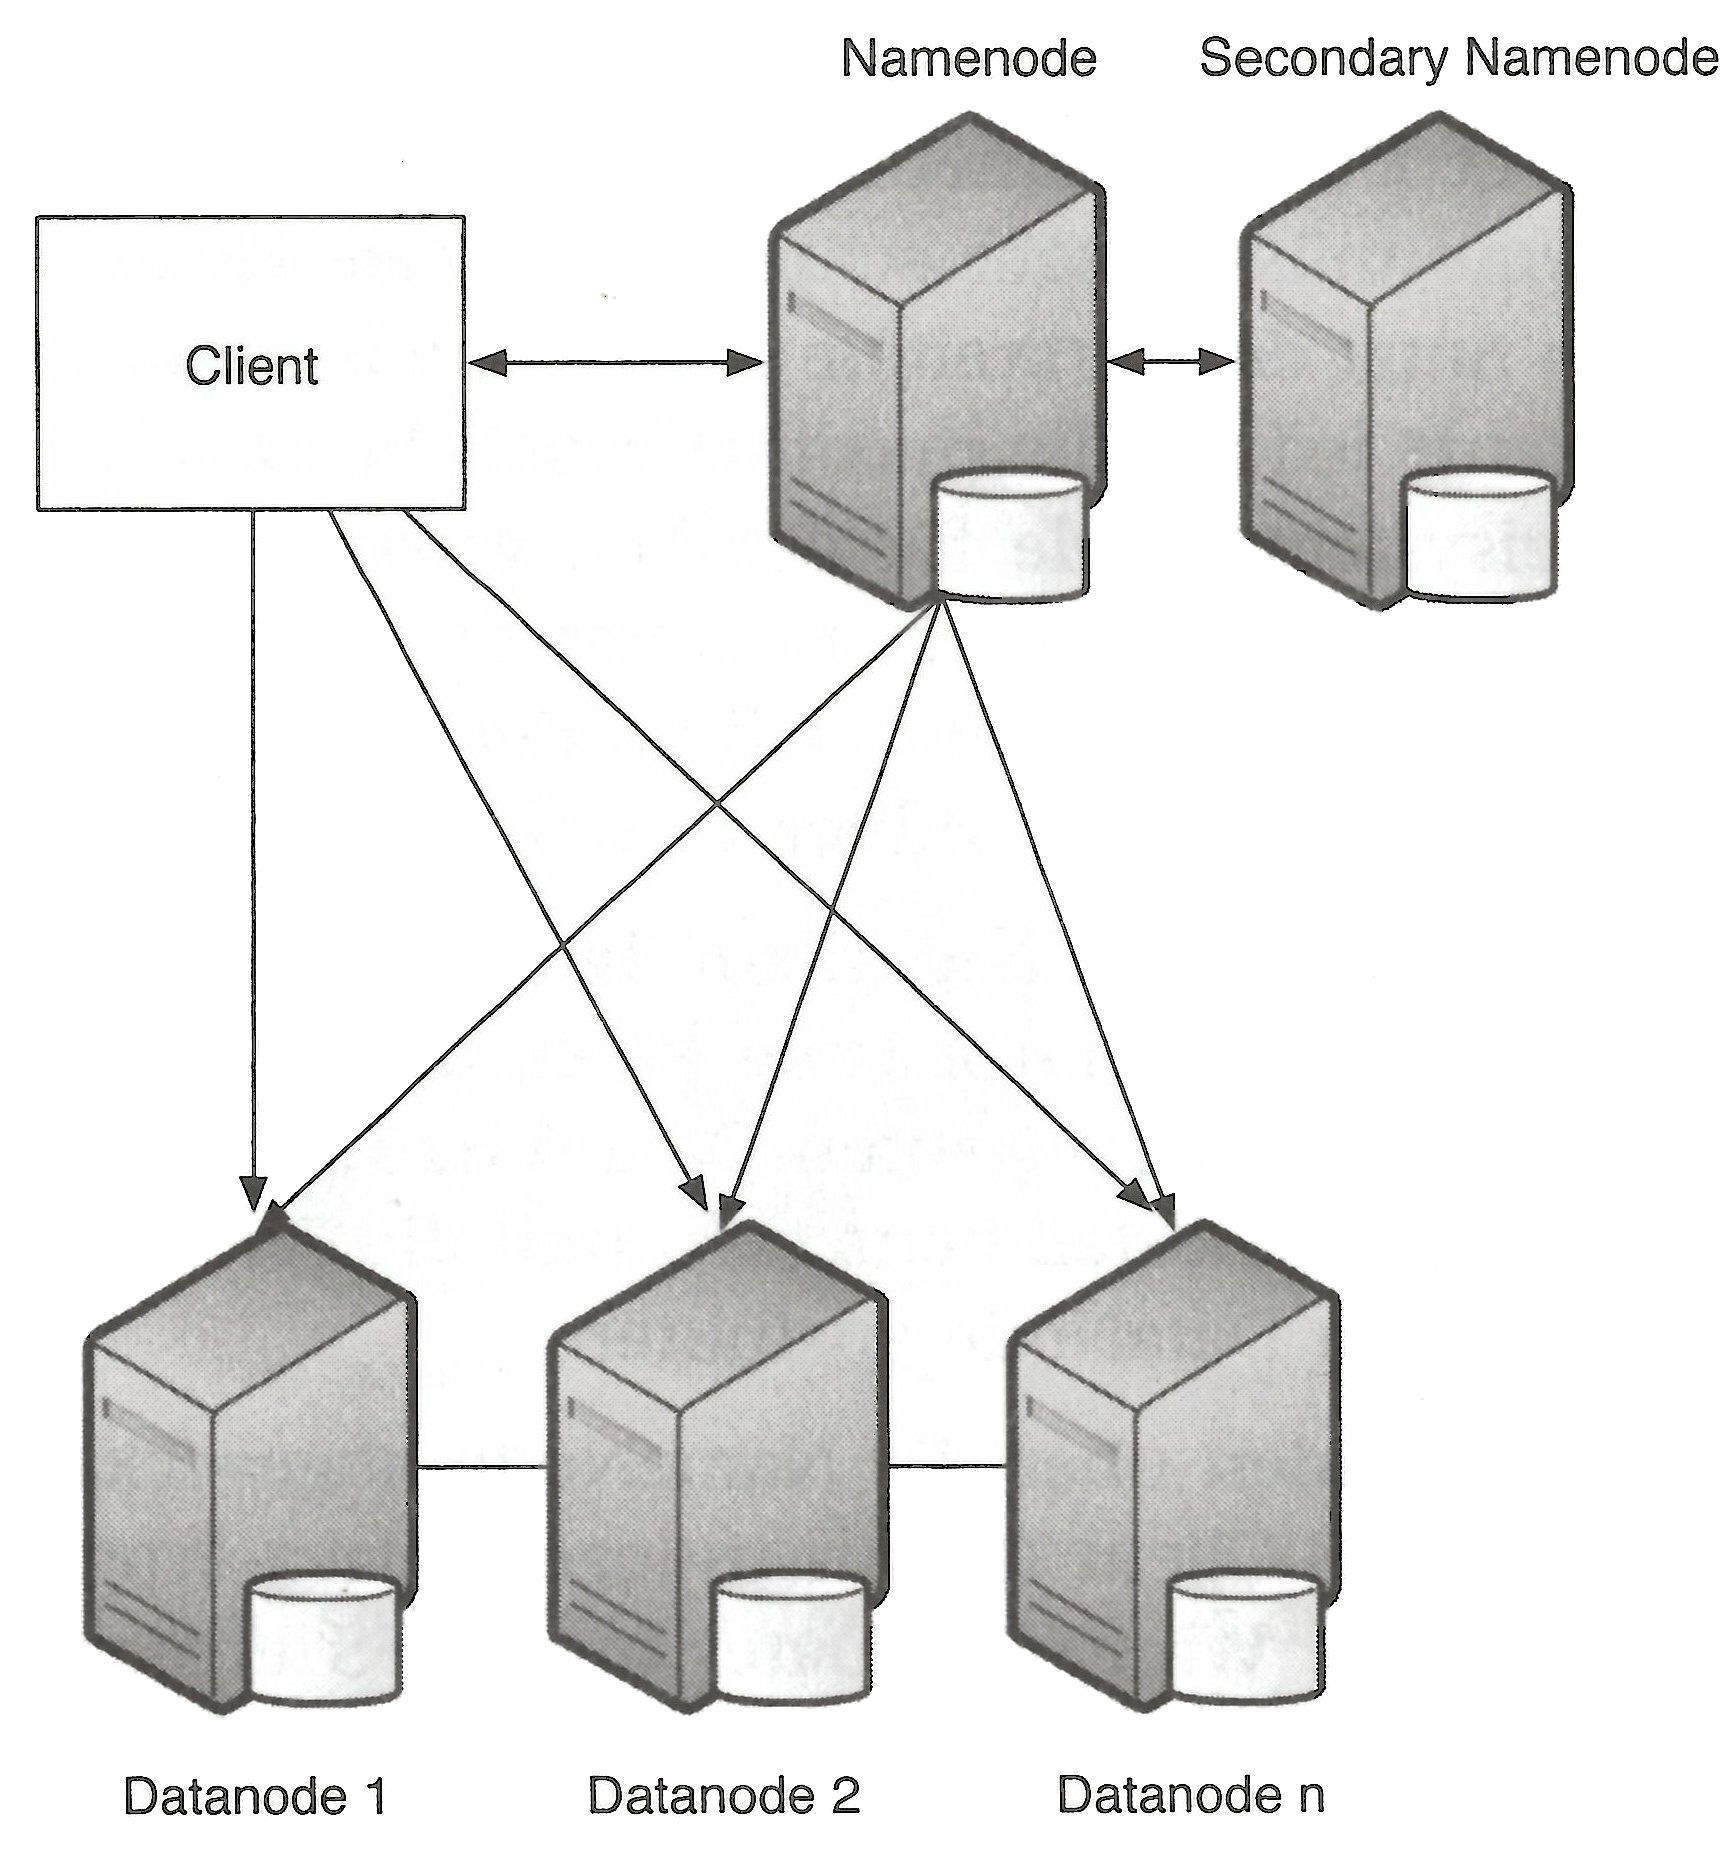
\includegraphics[scale=1.2]{HDFS_Architektur.png}
	\caption{HDFS Architektur-Schema\footnotemark}
	\label{fig:HDFSArchitekturSchema}
\end{figure}
\footnotetext{\cite[S. 23.]{Wartala.2012}}

\subsubsection{NameNodes}
Der NameNode kontrolliert und regelt alle Dateioperationen, welche auf das Dateisystem ausgeübt werden sollen. Er stellt den Master des Systems dar, und kümmert sich um die Speicherung der Dateinamen, Verzeichnisse und Zugriffe. Dabei koordiniert er die Verteilung der Dateiblöcke im Cluster und überwacht die ihm bekannten Slave Knoten (DataNodes). Der NameNode speichert lediglich Metainformationen über die im Dateisystem gespeicherten Daten. Die Daten selbst werden von ihm an die DataNodes weiter geleitet. Zusammengefasst sind die Aufgaben des NameNode:

\begin{itemize}
	\item Speicherung der Metadaten im Hauptspeicher
	\item Verteilung der Datenblöcke
	\item Überwachung der DataNodes, um Ausfälle oder beschädigte Daten schnell erkennen zu können.
\end{itemize}

Da alle Metadaten des Dateisystems im Hauptspeicher des NameNodes gehalten werden, ist die Anzahl der Dateien, die im \ac{HDFS} abgelegt werden können, begrenzt. Die Datenblöcke sind i.d.R. zwischen 64 und 128 \ac{MB} groß (im Gegensatz zu traditionellen Dateisystemen, welche mit Blöcken in der Größe 1 bis 64 \ac{KB}). Für die Verwaltung eines einzelnen Datenblocks benötigt der NameNode ca. 150 Byte. Bei einer Hauptspeichergröße von 1 \ac{GB} können i.d.R. mehr als 6 Mio. Dateien und Ordner verwaltet werden.\footcite[Vgl.][S. 24]{Wartala.2012}

Alle Anfragen an das \ac{HDFS} laufen über den NameNode. Dabei werden die Befehle von einem \ac{HDFS}-Client gesendet (Kommandozeile, Java-Programm, etc.). Die im Zuge der Bachelorarbeit programmierte Anwendung verwendet das Java \ac{API}, welches von Hadoop bereitgestellt wird.

\subsubsection{DataNodes}
DataNodes sind die Slave Knoten des Dateisystems, in welchen die Datenblöcke gespeichert werden. Sie besitzen keine Informationen über die Daten selbst. Aufgaben der DataNodes sind:

\begin{itemize}
	\item Verwaltung der einzelnen Dateisystem-Blöcke
	\item Dateisystem innerhalb einer Replikationskette (Replication chain)
	\item Zustandsinformationen (über sich selbst und die Daten) für NameNode bereitstellen
\end{itemize}

Zudem werden die MapReduce-Prozesse auf genau den Knoten ausgeführt, welche die benötigten Daten besitzen. DataNodes replizieren selbstständig die durch den NameNode übermittelten Daten an weitere DataNodes, wenn ihnen Dies durch den Master mitgeteilt wird. Zudem können sie, nach einer entsprechenden Anweisung des NameNodes, beschädigte Datenblöcke von anderen DataNodes kopieren und ersetzen.\footcite[Vgl.][S. 25 f.]{Wartala.2012}

%<Was ist ein verteiltes Dateisystem überhaupt und wozu braucht man es? Vergleich mit einem normalen Dateisystem?>

%\subsection{MapReduce-Framework}\label{subsec:MapReduceFramework}
%ACHTUNG. Vermutlich überflüssig da MapReduce bereits beschrieben wurde. Das Framework funktioniert nicht wirklich anders es stellt nur interfaces bereit damit die klassen stimmen.

\subsection{Abgrenzung - Was ist Hadoop nicht?}
Es gibt unterschiedliche Techniken für die Speicherung und Verarbeitung von Daten, mit ihren jeweiligen Stärken und Schwächen. Es gibt eine Reihe von Kritikern, welche dem MapReduce-Ansatz unterschiedlichste Mängel vorwerfen. Darunter u.a. das der Ansatz nicht wirklich innovativ und würde Funktionen wie Loadbalancing, Transaktionen oder auch Views vermissen.

Es ist daher wichtig zu wissen, was Hadoop nicht ist. Jede Technologie ist nur dann Sinnvoll, wenn sie der Aufgabe entsprechend eingesetzt wird. Für die Aufgaben, für welche Hadoop konzipierte wurde, sind keine Transaktionen oder Views notwendig. Diese Funktionalitäten werden bei relationalen Datenbanken (und deren Aufgaben) benötigt, nicht jedoch bei Hadoop.

%TODO: Abwägen ob dieser Absatz in das Kapitel "Was ist Hadoop" gehört. Meine Idee war, dass dieser Absatz die Abgrenzung zu relationalen Datenbanksystemen verdeutlichen sollte.
Laut Wartala gibt es eine Reihe von algorithmischen Problemlösungen, welche i.d.R. auf Hadoop besser ausgeführt werden können, als auf einem relationalen Datenbanksystem. Darunter unter anderem die Indexierung für Suchmaschinen, Text Mining, sowie die Analyse von Logfiles und Click-Streams.

Eine weitere Unterscheidung muss zu Systemen gemacht werden, welche in die Gruppe der \ac{EDA} bzw. \ac{CEP} Systeme fallen. Der Fokus von Hadoop liegt bei der Verarbeitung großer Datenmengen mittels Batch-Prozessen. Dieser Ansatz ist zu langsam für eine Real- oder Near-Time-Datenverarbeitung. Jedoch ist das Ziel eines \ac{EDA} oder \ac{CEP} Systems nicht die Abfrage gespeicherter Informationen, sondern die kontinuierliche Informationsbeschaffung, und haben somit eine vollkommen andere Funktion.

Eine letzte Abgrenzung muss zum sog. Grit Computing erfolgen. Hadoop konzentriert sich auf die Transformation von Schlüssel-Wert-Paaren innerhalb der MapReduce-Funktionen, und kann auf einer großen Zahl identischer Hardware installiert und ausfallsicher betrieben werden. Grid-Systeme dagegen verteilen Daten und Algorithmen auf einem niedrigeren Abstraktionsniveau. Dabei können einzelne Prozesse, über die im Grid Computing bekannte Schnittstelle \ac{MPI}, innerhalb eines Netzwerkes komplexere Nachrichten und Objekte austauschen. Grid-Systeme können somit mehr als nur Schlüssel-Wert-Paare verteilen. Eine solche komplexität ist bei Hadoop jedoch nicht notwendig.\footcite[Vgl.][S. 30-33]{Wartala.2012}

Das Fehlen dieser Funktionen zu kritisieren ist daher nicht sinnvoll. Es ist die Kombination unterschiedlicher Technologien, für ihren jeweiligen erdachten Zweck, die eine Architektur erfolgreich macht. \flqq Nicht ohne Grund betreibt der Erfinder des MapReduce-, \ac{GFS}- und BigTable-Ansatzes, Google, die weltgrößte MySQL-Installation.\frqq\footcite[S. 31]{Wartala.2012}

%<Was gehört alles zu Hadoop? Worauf zieht Hadoop ab? Warum verwende ich Hadoop statt es einfach selbst zu machen? Stärken und Schwächen aufzeigen.>

\subsection{Überlegungen zur Ausfallsicherheit von Hadoop}
Sowohl Wartala als auch Freiknecht, schreiben in ihren Büchern über die Ausfallsicherheit von Hadoop. Durch die Replikation eines Datenblocks auf unterschiedliche DataNodes, stehen die Daten selbst bei einem Ausfall eines Knotens zu Verfügung. Das Dateisystem kann so konfiguriert werden, dass es nicht nur über die Anzahl der DataNodes Kenntnis besitzt, sondern ebenfalls über deren Standort (anderer Server, Rack oder anderes Rechenzentrum).

In einer komplexeren Infrastruktur, mit mehreren DataNodes, verteilt auf unterschiedliche Racks, folgt Hadoop zwei grundsätzlichen Regeln bei der Replikation von Datenblöcken:

\begin{enumerate}
	\item Nur eine Replikation pro DataNode
	\item Nur maximal zwei Replikationen im gleichen Rack
\end{enumerate}

Die Knoten melden sich in regelmäßigen Abständen beim NameNode, um, zum einen, mitzuteilen dass sie noch aktiv sind, und um einen Abgleich der Datenblöcke mittels einer Checksumme vor zu nehmen. Sollte diese nicht stimmen, kann der NameNode dem betreffenden DataNode den Auftrag erteilen, den Datenblock von einem anderen Knoten zu kopieren. Dadurch wird der beschädigte Block ersetzt. Die Integrität der Daten ist somit durch die Replikation sehr sicher.

Es gibt jedoch einen großen Schwachstelle in Form des im System einmalig vorhandenen NameNodes. Dieser stellt einen \ac{SPOF} dar. Ein Ausfall des NameNode würde das gesamte Dateisystem lahm legen. Zudem besteht die Gefahr, dass, bei einem plötzlichen Ausfall des NameNode, die gespeicherten Metadaten beschädigt oder verloren gehen.

Aus diesem Grund muss der NameNode über entsprechende Sicherheitsvorkehrungen verfügen, um das Ausfallrisiko zu minimieren.

%<Verteilung der Replikationen über mehrere DataNodes in verschiedenen Racks, Single Point of Failor!>

%\section{Betrachten von Alternativen}
%Alternativen sowohl zu Hadoop als auch zu MapReduce selbst. Was gibt es in diesen Bereichen noch? Wie unterscheiden sich diese?
%TODO: Alternativen in 3.3 und 5.1 oder eher 5.4 betrachten/erwähnen

		
	% Planung
	%!TEX root = ../dokumentation.tex

\chapter{Planung}\label{cha:Planung}
Bevor mit die Entwicklung der Anwendung begonnen werden kann, müssen die Anforderungen, sowie Ziele und Umgebung festgelegt werden. Die exakte Planung eines ist notwendig, um eine qualitativ hochwertige, lösungsorientierte Anwendung zu entwickeln.

%Beschreiben worum es im Kapitel geht. Warum wird eine Planung gemacht? Was ist das Ziel der Planung?

\section{Anforderungen \& Produktleistungen}
<Schreiben wozu die Ziele gut sein sollen. welche form sollen sie haben. welchen zweck dienen sie usw. Zusätzlich schreiben warum manche aspekte wie die art der logs nicht definiert wurden oder manche ziele eher abstrakt sind>

\subsection{Anforderungen}
Im folgenden werden die Anforderungen beschrieben, welche an die fertige Anwendung gestellt werden. Bei der Definition von Anforderungen oder Zielen ist es hilfreich, sich gedanklich an das Ende des Projektes zu versetzen, und diese Situation dan zu beschreiben. Außerdem sollten alle Anforderungen "`smart"' sein, d.h., sie sind \textbf{s}peziefisch, \textbf{m}essbar, \textbf{a}ttraktiv, \textbf{r}ealistisch und \textbf{t}erminiert.\footcite[Vgl.][S. 48]{Bauer.2014}

Bei den folgenden Definitionen gibt es keine unterscheidung bei der Priorität. Alle Anforderungen müssen mit der fertigen Anwendung abgedeckt sein. Des weiteren handelt es sich um rein funktionale Anforderungen. 

\subsubsection{A001 - Formatunabhängige Analyse}\label{subsubsec:A001}
Die Analyse eines Logfiles muss unabhängig von dessen Format möglich sein. Alle textbasierten Formate (z.B. .txt, .log, .csv, usw.) müssen durch die Anwendung interpretierbar sein. Eine Umwandlung der Datei soll nicht stattfinden. Es wird davon ausgegangen, dass alle Logfiles UTF-8 codiert sind.

\subsubsection{A010 - Dynamisches Analyseverfahren}\label{subsubsec:A010}
Die Analyse eines Logfiles muss dynamisch sein, d.h., dass die Parameter der Analyse flexibel eingestellt werden können. Dies bezieht sich in erster linie auf relevante Muster, welche durch Reguläre Ausdrücke oder Keywords eingestellt werden können, und einen Zeitraum, in welchem die relevanten Muster liegen müssen.

\subsubsection{A020 - Konfigurierbarkeit}\label{subsubsec:A020}
Die Anwendung muss für jede  Ausführung individuell konfigurierbar sein. Die Konfiguration findet über eine Datei des Typs \textit{.properies} statt, welche zu Beginn der Ausführung durch die Anwendung geladen und interpretiert werden muss. Die Konfigurationswerte folgen der, für dieses Dateiformat üblichen, Formatierung. Jeder Eintrag besteht aus einem eindeutigen Schlüssel sowie einem dazu gehörenden Wert. Die Trennung erfolgt durch einen Doppelpunkt.

\subsubsection{A030 - Erweiterbarkeit}\label{subsubsec:A030}
Die Anwendung muss eine modularen Aufbau folgen, um eine einfache Erweiterbarkeit um eventuell folgende Features zu gewährleisten. Die einzelnen Komponenten müssen, soweit dies programmatisch möglich ist, über eine lose Kopplung besitzen. Dies soll sicherstelle, dass neue Komponenten hinzugefügt oder bestehende ausgetauscht werden können, ohne die Integrität der Anwendung zu gefärden.

%\begin{table}[h]
%	\centering
%	\begin{tabular}{| l | l | l | l | l |}
%		\hline
%		\rowcolor[HTML]{3531FF} 
%		\multicolumn{1}{|l|}{\cellcolor[HTML]{3531FF}{\color[HTML]{FFFFFF} {\bf \#ID}}} & \multicolumn{1}{l|}{\cellcolor[HTML]{3531FF}{\color[HTML]{FFFFFF} {\bf Name}}} & \multicolumn{1}{l|}{\cellcolor[HTML]{3531FF}{\color[HTML]{FFFFFF} {\bf Modul}}} & \multicolumn{1}{l|}{\cellcolor[HTML]{3531FF}{\color[HTML]{FFFFFF} {\bf Beschreibung}}} & \multicolumn{1}{l|}{\cellcolor[HTML]{3531FF}{\color[HTML]{FFFFFF} {\bf Priorität}}} \\ \hline
%		01 & Konfigurierbarkeit & Properties & Die Anwendung muss über eine .properties Datei konfigurierbar sein & 1 \\ \hline
%		02 &                                                                                      &                                                                                      &                                                                                      &                                                                                      \\ \hline
%		03 &                                                                                      &                                                                                      &                                                                                      &                                                                                     \\  \hline
%	\end{tabular}
%	\caption{My caption}
%	\label{my-label}
%\end{table}

\subsection{Produktleistungen}
Zusätlich zu den beschriebenen, funktionalen Anfordernen, werden weitere, nicht funktionale Leistungen definiert, welche durch von der fertigen Anwendung erfüllt werden müssen. Hierbei handelt es sich in erster linie um Richtwerte, welche sich i.d.R. auf die Performance der Anwendung beziehen.

\subsubsection{PL001 - Ausführungszeit}\label{subsubsec:PL001}
Die Ausführungszeit der Anwendung muss unter dem im folgenden definierten Richtwert liegen. Ist die einhaltung von diesem nicht möglich, muss eine alternative für den Verarbeitungsprozess implementiert werden, welche die Ergebnisse der Analyse in einer NoSQL-Datenbank speichert, welche dan durch ein Checkscript abgefragt werden kann.

Es ist nicht möglich einen festen Richtwert für die Ausführungszeit zu definieren, da dieser in Abhängigkeit zum Ausführungsinterval steht (z.B. wäre eine max. Ausführungszeit von einer Minute bei einem Interval von einer Minute nicht ausreichend). Aus diesem grund wird die maximale Ausführungszeit $t_e$, in abhängigkeit zum Interval $t_i$, wie folgt definiert:

\begin{equation}
t_e \leq \frac{t_i}{5} \quad \{t_e \in \mathbb{Q}^+\},\;\{t_i \in \mathbb{N}\} \label{equ:MaxAusführungszeit}
\end{equation}

\subsubsection{PL010 - Dateigröße}\label{subsubsec:PL010}
Die Anwendung muss in der lage sein, Logfiles bis zu einer größe von 500 \ac{MB} verarbeiten zu können. Größere Dateien dürfen, wenn dies noch nicht durch \ac{HDFS} selbst vorgenommen wurde, in mehrere Dateien, für die weitere Verarbeitung, zerlegt werden.

\section{Definition der Umgebung}
Die Programmierung der Anwendung erfolgt in der Programmiersprache Java, unter verwendung des Hadoop Frameworks für MapReduce in der Version 2.7.1. Die Entwicklung wird mit der \ac{IDE} \gls{NetBeans}, Version 8.0.2, durchgeführt. Für die Versionsverwaltung wird \gls{Git} eingesetzt. In der \ac{IDE} wird ein \gls{Maven}-Projekt erzeugt, um alle benötigten Bibliotheken automatisch, durch die \ac{IDE}, beziehen zu können.

%TODO: Datenbank definieren
Über die \ac{IDE} wird eine ausführtbare JAR-Datei erzeugt, welche auf dem Server mit Hadoop ausgeführt werden soll. Für die Ausführung wird Java in Version 1.7 benötigt.

Sollte sich im Verlauf der Entwicklung abzeichen, dass der Richtwert, welcher in \autoref{subsubsec:PL001} durch \autoref{equ:MaxAusführungszeit} definiert wurde, nicht eingehalten werden kann, so muss eine NoSQL-Datenbank für die Speicherung der Ergebnisse verwendet werden. In diesem Fall muss das entsprechende Datenbanksystem auf dem Server vorhanden sein.

Die anwendung wird durch das Hadoop Framework Version 2.7.1 ausgeführt. Es muss mindestens eine \textit{Single Node} Installation vorhanden sein. Es müssen die entsprechenden Rechte auf dem Dateisystem \ac{HDFS} gesetzt sein, um Dateien lesen und schreiben zu können.

%Welche Sprache wird verwendet? Auf welcher Plattform wird entwickelt? Welche Technologien werden eingesetzt.

%\section{Datenschutzrichtlinien}
%<Hier müssen die Datenschutzbestimmungen abgehandelt werden. Im normalfall wären IP Adressen personenbezogene daten und müssten geschützt werden. Es gibt da aber die außnahme in verbindung mit dem gesetz zur Vorratsdatenspeicherung. Darauf muss eingegangen werden um klar zu stellen unter welchen rechtlichen grundlagen die verarbeitung hier stattfinden kann. Dabei sollten auch die begriffe der anonymisierung und pseudonymisierung geklärt werden und was gemacht werden muss (wenn überhaupt).>
	
	% Setup
	%!TEX root = ../dokumentation.tex

\chapter{Setup}\label{cha:Setup}
Vor Beginn der Implementierung steht das Setup der Entwicklungsumgebung. Um die Anwendung testen zu können, wird eine \ac{VM} mit dem \ac{OS} Ubuntu verwendet. Auf diesem muss Hadoop installiert und konfiguriert sein. Dabe ist zu beachten, dass es sich um eine Single Node Installation handelt. Es wird also kein Clustering vorgenommen.

Auch in der \ac{IDE} muss ein Setup durchgeführt werden. Dabei handelt es sich, wie auch bei der Konfiguration der \ac{VM}, um Einstellungen, welche nicht im Zusammenhang mit der Umsetzung der Anwendung stehen. Die nachfolgenden Schritte werden so (oder ähnlich) für die Entwicklung aller Hadoop MapReduce Anwendungen vorgenommen.

<Einleitung in das Kapitel noch nicht komplett rund...>

\section{Installation \& Konfiguration}\label{sec:InstallationHadoop}
Die Installation des Testsystems findet auf einer Linux \ac{VM} mit Ubuntu Version 14.04.2 \ac{LTS} statt, und wird nach der durch Freiknecht beschriebenen Anleitung durchgeführt. 

\subsection{Einrichten eines dedizierten Hadoop-Users}
Dabei wird zunächst ein eigener User, sowie eine eigene Gruppe, für Hadoop angelegt. Dies wird aus Sicherheitsgründen gemacht, da keine Anwendung als Root-User ausgeführt werden darf.

Zusätzlich wird ein \ac{SSH} Zugang für den User angelegt. Hierzu nennt Freiknecht als Gründe zum einen, dass später bei der Verwendung eines Hadoop-Clusters, die Systeme miteinander kommunizieren müssen, und zum anderen, dass auch vom Hostsystem Dateien auf der \ac{VM} abgelegt werden. Für den \ac{SSH}-Zugang muss ein Schlüssel nach dem Verfahren von \ac{RSA} für den User erzeugt und bei den autorisierten Schlüsseln abgelegt werden. Abschließend, um den Host zu den bekannten Systemen hinzuzufügen, muss der Hadoop User eine erstmalige Verbindung herstellen.\footcite[Vgl.][S. 30 f.]{Freiknecht.2014}

\autoref{lis:KonfHadoopUser} zeigt die Kommandozeilen Befehle für die gerade beschriebenen Aktionen. \\

\begin{lstlisting}[language=bash, caption={Konfiguration des Hadoop Users}, label=lis:KonfHadoopUser]
# Create usergroup and user
sudo addgroup hadoop
sudo adduser -ingroup hadoop hduser

# login as hadoop user and create rsa key
su - hduser
ssh-keygen -t rsa -P ""

# add to authorized keys
cat $HOME/.ssh/id_rsa.pub >> $HOME/.ssh/authorized_keys

# Initial login on host via ssh
ssh localhost
\end{lstlisting}

\subsection{Installation des Hadoop Frameworks}
Nachdem der dedizierter User angelegt wurde, kann die Installation von Hadoop selbst durchgeführt werden. Hierzu wird zunächst die aktuelle Version von Hadoop in das Verzeichnis \textit{/usr/local} heruntergeladen, entpackt und umbenannt nach \textit{hadoop}. Zuletzt werden die benötigten Berechtigungen für den dedizierten User gesetzt (\autoref{lis:HerunterladenUndEntpacken}). Im Gegensatz zur Anleitung von Freiknecht wird die aktuelle Hadoop Version 2.7.1 statt 2.2.0 verwendet. \\

\begin{lstlisting}[language=bash, caption={Herunterladen und entpacke von Hadoop}, label=lis:HerunterladenUndEntpacken]
$ cd /usr/local
$ sudo wget http://apache.openmirror.de/hadoop/common/current
            /hadoop-2.7.1.tar.gz
$ sudo tar xfz hadoop-2.7.1.tar.gz
$ sudo mv hadoop-2.7.1 hadoop
$ sudo chown -R hduser:hadoop hadoop
\end{lstlisting}

Da Hadoop in einem extra Verzeichnis installiert wurde, müssen für den User noch eine Reihe von Umgebungsvariablen gesetzt werden. Diese werden der Datei \textit{.bashrc}, welche im Home-Verzeichnis des Users liegt, hinzugefügt. \\

\begin{lstlisting}[language=bash, caption={Umgebungsvariablen für Hadoop}, label=lis:Umgebungsvariablen]
# Java
export JAVA_HOME=/usr/lib/jvm/java-7-openjdk-amd64

# Hadoop
export HADOOP_INSTALL=/usr/local/hadoop
export PATH=$PATH:$HADOOP_INSTALL/bin
export PATH=$PATH:$HADOOP_INSTALL/sbin
export HADOOP_MAPRED_HOME=HADOOP_INSTALL
export HADOOP_COMMON_HOME=HADOOP_INSTALL
export HADOOP_HDFS_HOME=HADOOP_INSTALL
export HADOOP_YARN_HOME=HADOOP_INSTALL
\end{lstlisting}

Abschließend muss die Installation von Hadoop getestet werden, indem der Befehl \textit{hadoop version} in der Kommandozeile ausgeführt wird. \autoref{fig:ErgebnisKomandozeileneingabe} zeigt das Ergebnis der Kommandozeileneingabe. Die Ausgabe bestätigt die erfolgreiche Installation.\footcite[Vgl.][S. 32 f.]{Freiknecht.2014}

\begin{figure}[h]
	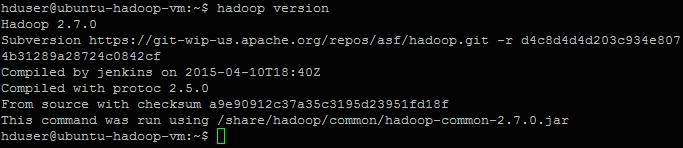
\includegraphics[width=1\textwidth]{hadoop_version.png}
	\caption{Ergebnis für die Kommandozeileneingabe \textit{hadoop version}}
	\label{fig:ErgebnisKomandozeileneingabe}
\end{figure}

\subsection{Konfiguration für Pseudo-Distributed Umgebung}
Hadoop kann als Single Node Installation auch in einer Pseudo-Distributed Umgebung laufen, in welcher jeder Hadoop Deamon als eigenständiger Java-Prozess ausgeführt wird. Um dies zu ermöglichen, sind weitere Konfigurationen notwendig, da für diese Umgebung \ac{HDFS} aktiviert wird.

Die Konfiguration wird nach der Dokumentation von Apache durchgeführt. Dabei werden zunächst Einstellungen in den Dateien \textit{core-site.xml} und \textit{hdfs-site.xml}, welche im Verzeichnis \textit{etc/hadoop} zu finden sind, vorgenommen. \autoref{lis:KonfCoreSite} und \autoref{lis:KonfHDFSSite} zeigen die entsprechenden Konfigurationen. \\

\pagebreak
\begin{lstlisting}[language=XML, caption=Konfiguration in der core-site.xml, label=lis:KonfCoreSite]
<configuration>
	<property>
		<name>fs.defaultFS</name>
		<value>hdfs://localhost:9000</value>
	</property>
</configuration>
\end{lstlisting}

\begin{lstlisting}[language=XML, caption=Konfiguration in der hdfs-site.xml, label=lis:KonfHDFSSite]
<configuration>
	<property>
		<name>dfs.replication</name>
		<value>1</value>
	</property>
</configuration>
\end{lstlisting}

Um die Installation zu testen, muss zunächst eine Formatierung der Knoten vorgenommen werden. Erst nach einer Formatierung ist der Start des Dateisystems möglich. Über den Befehl \textit{jps} ist die Anzeige aller laufenden Java-Prozesse möglich. \autoref{lis:TestenDerKonf} zeigt die hierfür notwendigen Befehle. Hadoop bietet zusätzlich ein Web-Interface für die Knoten, welches über \textit{http://localhost:50070/} aufgerufen werden kann. Ein Screenshot des Interfaces ist im Anhang zu finden.\footcite[Vgl.][]{ApacheHadoopDoku.2015} \\

\begin{lstlisting}[caption=Test der Konfiguration, label=lis:TestenDerKonf]
$ bin/hdfs namenode -format
[...]
$ sbin/start-dfs.sh
[...]
$ jps
1277 DataNode
1337 NameNode
2311 Jps
1533 NodeManager
1566 SecondaryNameNode
$ sbin/stop-dfs.sh
[...]
\end{lstlisting}

%<Beschreibung der Installation. Was muss dabei beachtet werden? Was ist wichtig? Was wird ignoriert?>

\section{Anlegen eines neuen Maven Projektes}
Um eine Anwendung zu Programmieren, welche mit dem Hadoop Framework ausgeführt werden soll, müssen die entsprechenden Klassen von Hadoop im Build enthalten sein. Die benötigten Bibliotheken sind über \gls{Maven} beziehbar. \gls{NetBeans} bietet die Möglichkeit, ein neues Projekt direkt als \gls{Maven}-Projekt anzulegen (\autoref{fig:NewMavenProject01}).

\begin{figure}[h]
	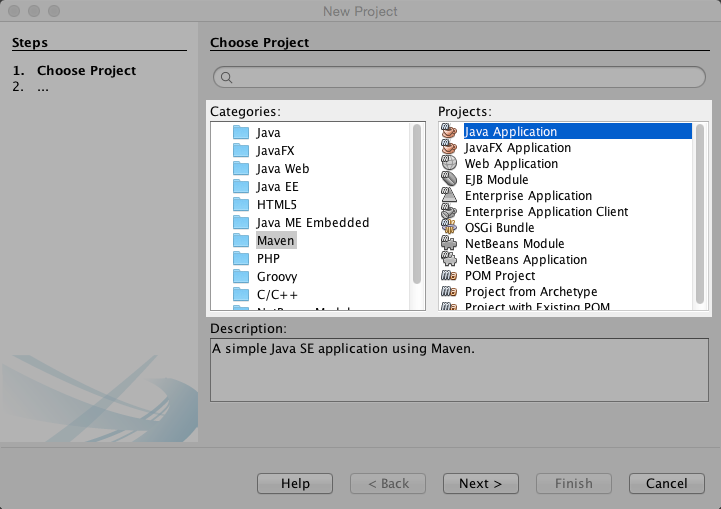
\includegraphics[width=1\textwidth]{NewMavenProject_01.png}
	\caption{Anlegen neuer Maven Java Application in NetBeans}
	\label{fig:NewMavenProject01}
\end{figure}

Charakteristisch für ein \gls{Maven}-Projekt ist das \ac{POM}, eine XML-Repräsentation des Projektes, welche in der \textit{pom.xml} gespeichert wird. Diese ist direkt im Projektverzeichnis des Dateisystems, oder im \textit{Project Files} Verzeichnis, in der \textit{Projects}-View von \gls{NetBeans} zu finden.

Um die zu Hadoop gehörenden Bibliotheken einzubinden, müssen diese im Knoten \textit{dependencyManagement/dependencies} angelegt sein. \autoref{lst:PomXML} zeigt die Für dieses Projekt eingebundenen Bibliotheken in der \textit{pom.xml}.

Für jede \textit{dependency} werden drei Angaben benötigt. Die \textit{groupId} bezeichnet das Paket, in welchem die Bibliothek zu finden ist und \textit{artifactId} enthält den Namen innerhalb des Paketes. Über die Angabe der \textit{version} ist die Einbindung unterschiedlicher Releases einer Bibliothek möglich. Dies ist notwendig, da bestehende Anwendungen eventuell  mit den neusten Versionen einer Bibliothek kompatibel sind.

Bis auf die Bibliothek \textit{hadoop-core} werden alle mit der Version 2.7.1 angegeben. Dies liegt darin begründet, dass sich der Core von Hadoop seit Version 1.2.1 nicht mehr verändert hat. \\

\begin{lstlisting}[caption=Auszug aus der \textit{pom.xml},label=lst:PomXML]
<dependencyManagement>
	<dependencies>
		<dependency>
			<groupId>org.apache.hadoop</groupId>
			<artifactId>hadoop-hdfs</artifactId>
			<version>2.7.1</version>
		</dependency>
		<dependency>
			<groupId>org.apache.hadoop</groupId>
			<artifactId>hadoop-auth</artifactId>
			<version>2.7.1</version>
		</dependency>
		<dependency>
			<groupId>org.apache.hadoop</groupId>
			<artifactId>hadoop-common</artifactId>
			<version>2.7.1</version>
		</dependency>
		<dependency>
			<groupId>org.apache.hadoop</groupId>
			<artifactId>hadoop-core</artifactId>
			<version>1.2.1</version>
		</dependency>
	</dependencies>
</dependencyManagement>
\end{lstlisting}

Um zu verhindern, dass, bei jeder Ausführung der später erzeugten Jar-Datei, die Angabe der \textit{Main Class} erfolgen muss, kann diese über ein \gls{Plugin} konfiguriert werden. Hierzu ist eine zusätzliche Angabe in der \textit{pom.xml}, unter dem Knoten \textit{build/plugins} notwendig, welche in \autoref{lst:MainClassDefinition} zu sehen ist. \\

\pagebreak
\begin{lstlisting}[caption=Definition der \textit{Main Class} des Projektes,label=lst:MainClassDefinition]
<plugin>
	<groupId>org.apache.maven.plugins</groupId>
	<artifactId>maven-jar-plugin</artifactId>
	<version>2.4</version>
	<configuration>
		<archive>
			<manifest>
				<mainClass>com.hszuesz.logfileanalyzer.Main</mainClass>
			</manifest>
		</archive>
	</configuration>
</plugin>
\end{lstlisting}

Zuletzt wurde für dieses Projekt eine Modifikation für die Generierung der Javadocs vorgenommen, um auch privat deklarierte Methoden mit zu erzeugen. \autoref{fig:JavaDocMod} zeigt, wo die notwendige Modifikation in \gls{NetBeans} erfolgen muss.

\begin{figure}[h]
	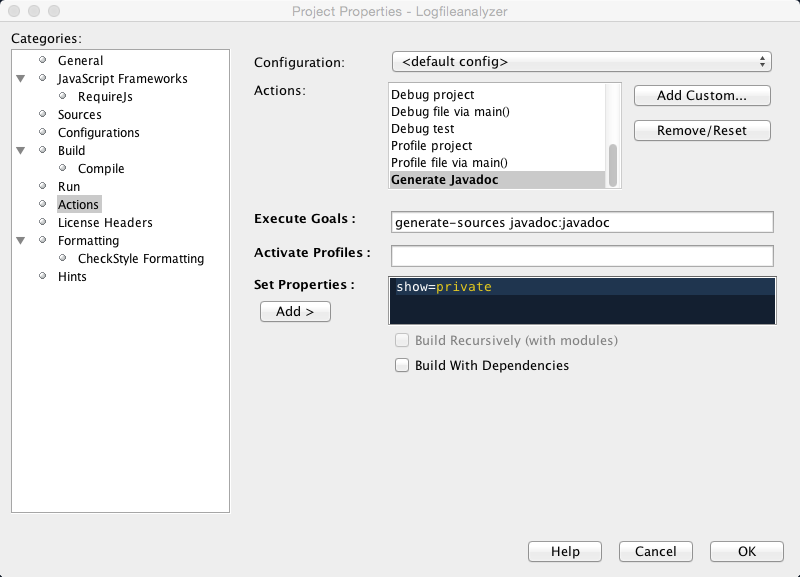
\includegraphics[width=1\textwidth]{NewMavenProject_03.png}
	\caption{Modifikation für Javadoc Generator}
	\label{fig:JavaDocMod}
\end{figure}

%<Noch ein Arbeitstitel. Hier soll es in erster Linie darum gehen wie man ein Projekt für die Entwicklung einer Java Anwendung anlegt, welche Hadoop MapReduce verwenden soll. Maven sollte aus dem Titel raus, da das noch nicht ein mal bis hier hin erwähnt wurde (außer vielleicht kurz in der Definition der Umgebung). Maven muss beschrieben werden, da es nicht ohne weiteres möglich ist eine Hadoop Anwendung zu schreiben ohne Maven.>
	
	% Umsetzung
	%!TEX root = ../dokumentation.tex

\chapter{Umsetzung}\label{cha:Umsetzung}
<Allgemeine Beschreibung des Inhalts des Kapitels.>

\section{Implementierung von Properties}
<Beschreibung wie Properties programmiert werden. Wie werden diese in der Anwendung umgesetzt? Welche Rolle spielen Properties für den generischen Teil der Anwendung?>

\section{Grundlagen für Datenverarbeitung}
<Beschreibung der Entwicklung für die Grundlagen zur Datenverarbeitung. Welche Klassen werden dabei verwendet? Welches System liegt dahinter? Warum dieses System? Dabei nicht nur auf die Speicherung von Daten eingehen sondern auch auf das Lesen von Dateien.>

\section{Bestimmung des Aufbaus der Logfiles}
<Wie sehen die Logfiles aus? Welche Formate haben sie? Welche rolle spielen diese bei der Datenverarbeitung? Welche Informationen sind die richtigen Informationen?>

\section{Implementierung von MapReduce}
<Beschreibung vom Kern der Anwendung. Wie wird der Algorithmus umgesetzt? Welche Klassen/Methoden sind notwendig? Wie unterscheidet sich die Implementierung bei unterschiedlichem Input. Spielt das überhaupt eine Rolle oder muss es nur Text sein? Welches Ergebnis bekommt man und in welcher Form?>
	
	% Schlussbetrachtung
	%!TEX root = ../dokumentation.tex

\chapter{Projektabschluss, Fazit \& Ausblick}\label{cha:Schlussbetrachtung}
<Projektabschluss. Worum geht es hier? Warum muss eine Schlussbetrachtung gemacht werden? Welche Schritte werden dabei durchgeführt?>

\section{Vergleich der Anwendung mit den Zielen}
Der Erfolg (oder Misserfolg) eines Projektes wird i.d.R. an dem sog. Erfüllungsgrad gemesssen. Dieser wird bestimmt, indem ein Abgleich, der zuvor definierten Ziele mit den Funktionen der fertigen Anwendung, vorgenommen wird.

Im Folgenden soll der Erfüllungsgrad für die vorliegende Anwendung bestimmt werden. Dabei muss beachtet werden, dass dieser lediglich eine Aussage über die Anwendung, nicht jedoch über die geschriebene Arbeit selbst trifft. Der Erfolg (oder Misserfolg) der Arbeit selbst wird in \autoref{sec:Fazit} festgestellt.

\subsection{Abgleich der funktionalen Anforderungen}
Im Folgenden werden die in \autoref{subsec:Anforderungen} definierten, funktionalen Anforderungen mit der fertigen Anwendung abgeglichen. Die Bewertung wird in drei Stufen durchgeführt. Diese sind erfüllt (3), teilerfüllt (2) und unerfüllt (1).

\subsubsection{A001 - Formatunabhängige Analyse (3)}
Die Verarbeitung der Logfiles wird ohne eine Umformung der Einträge durchgeführt. Es sind alle textbasierten Dateiformate analysierbar. Komplexere Daten sind, unter Implementierung einer entsprechenden \textit{InputFormat} Klasse, ebenfalls einlesbar.

\subsubsection{A010 - Dynamisches Analyseverfahren (3)}
Die Parameter der Analyse sind über die Konfigurationsschnittstelle flexibel. Suchmuster und Mappingverfahren sind über die entsprechenden Properties frei konfigurierbar.

\subsubsection{A020 - Konfigurierbarkeit (3)}
Die Anwendung ist über drei Stufen frei konfigurierbar. Es werden Dateien des Typs \textit{.properties} verwendet. Die Standardeinstellungen sind für jeden Programmlauf individuell anpassbar.

\subsubsection{A030 - Erweiterbarkeit (3)}
Durch die modulare Architektur des Programms und der hohen Flexibilität durch die Konfigurationsschnittstelle, sind Erweiterungen schnell und Einfach implementierbar. Da die Angabe, der zu verwendenden Klassen, immer mit dem vollständigen Paket erfolgen muss, ist ein Einbinden und Verwenden von externen Bibliotheken ohne Einschränkungen möglich.

\subsection{Abgleich der Produktleistungen}
Nach den funktionalen Anforderungen muss ebenfalls ein Abgleich der Anwendung mit den in \autoref{subsec:Produktleistungen} definierten Produktleistungen erfolgen. Dabei werden die gleichen Stufen wie beim Abgleich der funktionalen Anforderungen verwendet.

\subsubsection{PL001 - Ausführungszeit (2)}
Die maximale Laufzeit der Anwendung wurde durch \autoref{equ:MaxAusführungszeit} in \autoref{subsubsec:PL001} definiert. Nach der Entwicklung wurde, durch die Durchführung von Anwendungstests, eine Minimallaufzeit von $\approx 8$ Sekunden ermittelt. Dies ist auf einen Konstanten Zeitfaktor zurückzuführen, welcher bedingt wird durch das Starten der Anwendung innerhalb des Hadoop Frameworks.

Aus diesem Grund wird diese Produktleistung lediglich als teilerfüllt angesehen. Für Analysen mit einem Intervall von weniger als 40 Sekunden, wird die maximale Laufzeit überschritten.

\subsubsection{PL010 - Dateigröße (3)}
Die Vorgabe, Logfiles mit einer Größe von bis zu 500 \ac{MB}, ohne einen Split zu verarbeiten wird vollständig erfüllt. Erst ab einer Größe von ca. 1 \ac{GB} werden durch die Anwendung Splits erzeugt und parallel verarbeitet. 

\subsection{Zusammenfassung}
Abschließend wurde festgestellt, dass alle funktionalen Anforderungen vollständig erfüllt werden konnten. Bei den Produktleistungen gibt es lediglich eine teilerfüllung bei der maximalen Laufzeit der Anwendung.

Die Entwickelte Anwendung genügt den definierten Zielen. Das Projekt kann somit als Erfolgreich gewertet werden. 

%<Welche Ziele wurden erfüllt? Welche nicht? Alles bezogen auf die Anwendung nicht auf die Bachelor Arbeit! Wo gab es Abweichungen? Wenn ja, warum gab es die?>

%\section{Proof of Concept}
%<Dokumentation einer kompletten Durchführung der Anwendung von Anfang bis Ende. Aufzeigen der Ergebnisse. Funktioniert die Anwendung?>

\section{Fazit}\label{sec:Fazit}
Das Ziel der Arbeit, durch die Anwendung des MapReduce Verfahrens, schneller, bessere Informationen über den Zustand des Systems zu erhalten, konnte nicht vollständig erfüllt werden. Es wurde zwar eine prototypische Anwendung geschrieben, welche, mittels MapReduce, textbasierte Logfiles analysieren kann, jedoch nicht in einem dem Ziel entsprechenden Zeitraum.

Bei den durchgeführten Anwendungstests wurde ein konstanter Faktor von $\approx 8$ Sekunden festgestellt, welcher durch das Starten der Anwendung in Hadoop verursacht wird. In Verbindung mit dem Ziel, dass die Laufzeit der Analyse maximal $\sfrac{1}{5}$ des Ausführungsintervalls betragen sollte, bedeutet dies, dass nur Analysen mit einem Intervall von 40 Sekunden oder größer durchgeführt werden können. Dies ist für eine Real-/Neartime Analyse ein zu großer Intervall.

Es konnte jedoch gezeigt werden, dass sich, mit steigender Anzahl der zu verarbeitenden Einträge, die Ausführungskosten und die Effizienz von MapReduce stark verbessern. Die Verarbeitung von sehr großen Datenmengen ($\geq10^6$) ist die eigentliche Stärke des Modells.

Durch die Entwicklung der Applikation wurden nicht nur wertvolle Kenntnisse über die Funktionsweise des MapReduce Modells gewonnen, sondern auch Erfahrungen für die Arbeit im BigData-Bereich gesammelt werden.

Zudem wird durch die Anwendung, anstatt einer Verbesserung der Real-/Neartime Analyse der Infrastruktur, ein neues Werkzeug für Langzeitanalysen bereitgestellt (bzw. können alle Analysen mit einem Intervall $\geq$ 40 Sekunden durchgeführt werden).

Durch die modulare Entwicklung lässt sich die Applikation leicht erweitern. Die generische Struktur der Konfiguration ermöglicht zudem individuelle Anpassungen, wodurch eine Vielzahl unterschiedlicher Informationen gewonnen werden können.

Obwohl das eigentliche Ziel nicht erreicht wurde, kann die Arbeit aufgrund der gewonnenen Erkenntnisse und der entwickelten Applikation als Erfolg angesehen werden. Sowohl das Wissen über die Arbeitsweise von MapReduce als auch die Anwendung selbst stellen wertvolle Werkzeuge für zukünftige Analysen dar.

%<Fazit ziehen über das Projekt und die Arbeit. Welche Erkenntnisse wurden gewonnen? Was hat gut/schlecht funktioniert? Wurden die eigenen Erwartungen erfüllt oder nicht? War das Projekt erfolgreich?>

\section{Ausblick}\label{sec:Ausblick}
Vor Inbetriebnahme des Logfileanalyzers sollte eine Laufzeitanalyse, nach dem in \autoref{subsec:Laufzeitanalyse} beschriebenen Verfahren, auf dem Zielsystem durchgeführt werden. Daraus sollten sich neue Erkenntnisse bezüglich der Geschwindigkeit von MapReduce auf einem tatsächlichen System ergeben und somit das Einsatzgebiet des Programms klar werden.

Um das vollständige Potenzial der Anwendung ausnutzen zu können, sollte eine Änderung der Infrastruktur vorgenommen werden. Wie in \autoref{subsec:Infrastruktur} beschrieben wurde, werden die Logfiles aktuell auf einem \ac{NFS} abgelegt, und über einen mount an den Infrastrukturserver gebunden. Dies hat den Nachteil, dass die zu analysierenden Daten zunächst in ein dort laufendes \ac{HDFS} übertragen werden müssen.

Aus diesem Grund sollte das bestehende \ac{NFS} durch ein \ac{HDFS} ersetzt werden. Wenn dies erfolgt ist, kann die Grundidee von Hadoop, die Anwendung zu den Daten zu bringen, statt die Daten zur Anwendung, vollständig umgesetzt werden.

Um spezifischere Analysen durchführen zu können, sollten weitere \textit{Mapper}, sowie \textit{InputFormat} und \textit{RecordReader} Klassen entwickelt werden da diese die Grundlage für neue Analyseverfahren und der Verarbeitung weiterer Dateiformate bilden.

%<Welche Möglichkeiten bieten sich in der Zukunft? Was kann noch erreicht werden? Was bleibt offen? Welche nächsten Schritte sollte man gehen?>
	
	% Fazit
	%!TEX root = ../dokumentation.tex

\chapter{Fazit}\label{cha:Fazit}

\section{Ausblick}\label{sec:Ausblick}

	% Inhalt
	%\foreach \i in {01,02,03,04,05,06,07,08,09,...,99} {%
	%	\edef\FileName{content/\i kapitel}%
	%		\IfFileExists{\FileName}{%
	%			\input{\FileName}
	%		}
	%		{%
	%			%file does not exist
	%		}
	%}

	\clearpage
		
	\pagenumbering{roman}

	% Literaturverzeichnis
	\cleardoublepage
	\printbibliography

	% Glossar
	\printglossary[style=altlist,title=\langglossar]
	
	% sonstiger Anhang
	\clearpage
	\appendix
	% !TeX root = ../dokumentation.tex

\addchap{\langanhang}

{\Large
\begin{enumerate}[label=\Alph*.]
	\item Screenshot NameNode Web-Interface
	\item List of CD Contents
	\item CD 
\end{enumerate}
}
\pagebreak
\section*{A. Screenshot NameNode Web-Interface}
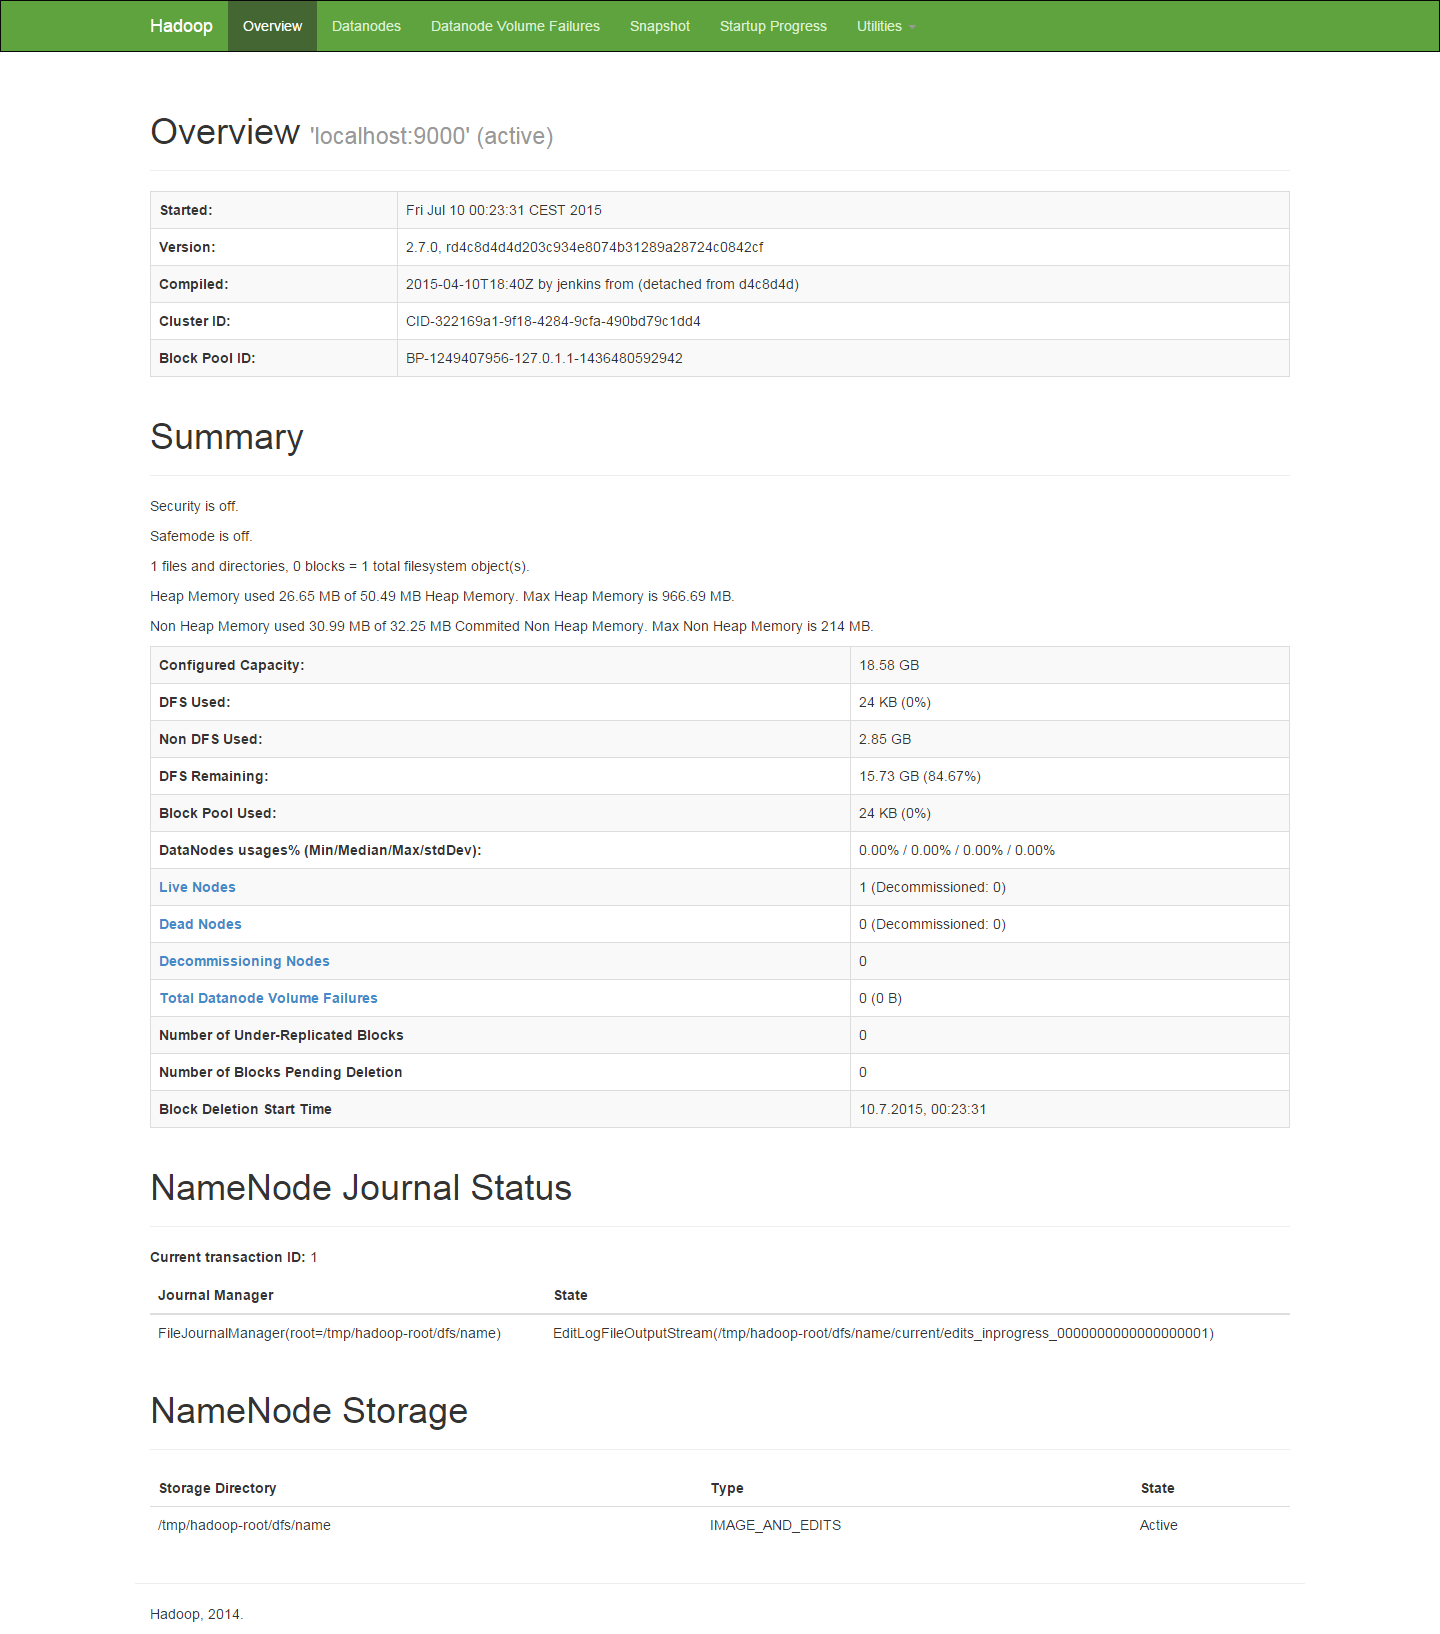
\includegraphics[width=1\textwidth]{NameNodeWebInterface.png}
\pagebreak
\section*{B. List of CD Contents}
\begin{tabbing}
	mm \= mm \= mmmmmmmmmmmmmmmm \= \kill
	$\vdash$ \textbf{Literature/} \\ 
	| \> $\vdash$ \textbf{Citavi-Project(incl pdfs)/} \> \> $\Rightarrow$ \textit{Citavi (bibliography software) project with}\\
	| \> | \> \> \textit{almost all found sources relating to this report.} \\
	| \> | \> \> \textit{The PDFs linked to bibliography items therein} \\
	| \> | \> \> \textit{are in the sub-directory `CitaviFiles'}\\
	| \> | \>  -- bibliography.bib  \> $\Rightarrow$ \textit{Exported Bibliography file with all sources}\\
	| \> | \>  --	Studienarbeit.ctv4  \>  $\Rightarrow$ \textit{Citavi Project file}\\
	| \> | \>  $\vdash$ \textbf{CitaviCovers/} \>  $\Rightarrow$ \textit{Images of bibliography cover pages}\\
	| \> | \>  $\vdash$ \textbf{CitaviFiles/} \> $\Rightarrow$ \textit{Cited and most other found PDF resources}\\ %\llcorner
	| \> $\vdash$ \textbf{eBooks/} \\
	| \> $\vdash$ \textbf{JournalArticles/} \\
	| \> $\vdash$ \textbf{Standards/}\\
	| \> $\vdash$ \textbf{Websites/} \\ %\llcorner
	|\\
	$\vdash$ \textbf{Presentation/} \\
	| \>  --presentation.pptx\\
	| \>  --presentation.pdf\\
	|\\
	$\vdash$ \textbf{Report/} \\ %\llcorner
	\>  -- Aufgabenstellung.pdf\\
	\>  -- Studienarbeit2.pdf\\
	\>  $\vdash$ \textbf{Latex-Files/}   $\Rightarrow$ \textit{editable \LaTeX~files and other included files for this report}\\ %\llcorner
	\> \>  $\vdash$  \textbf{ads/}   	\> $\Rightarrow$ \textit{Front- and Backmatter}\\
	\> \>  $\vdash$  \textbf{content/}  \> $\Rightarrow$ \textit{Main part}\\
	\> \>  $\vdash$  \textbf{images/}   \> $\Rightarrow$ \textit{All used images}\\
	\> \>  $\vdash$  \textbf{lang/}  \> $\Rightarrow$ \textit{Language files for \LaTeX~template}\\ %\llcorner
\end{tabbing}

	
\end{document}
